% !TeX root = ../main.tex
\chapter{系統架構與方法}

    本研究所設計之系統系利用超音波對麥克風造成的非線性響應輸出與自適應噪音消除高關聯度噪音等特性。
來嘗試解決在部署麥克風干擾器的場域裡無法取得有效聲學紀錄的問題。
同時藉由密碼系統的機密性與不可否認性,發展一套以其為基礎的會談錄音存取控制機制。
透過上述機制的結合,能夠使在部署超音波麥克風干擾器的會談情境中,於會談結束後,允許特定參與者得以取得有效之聲音記錄。


\section{符號定義}

    本研究設計之系統所使用符號與其意義如表 \ref{table:symbol} 所示。

\rowcolors{1}{white}{whitesmoke}
\begin{longtable}{c l}
    \hiderowcolors
    \caption{符號定義表} \label{table:symbol} \\

    \hiderowcolors
    \hline
    \multicolumn{1}{c}{\bf{符號}} & \multicolumn{1}{c}{\bf{釋義}} \\
    \hline
    \endfirsthead

    \hiderowcolors
    \multicolumn{1}{c}{\bf{符號}} & \multicolumn{1}{c}{\bf{釋義}} \\
    \hline
    \endhead

    \hiderowcolors
    \hline
    \endlastfoot

    \showrowcolors
    \DEFattenderAll   & 系統角色-會談參與者 (Attender) \\
    \DEFownerAll      & 系統角色-會談主持者 (Owner) \\
    \DEFmeetingbox    & 系統角色-會談終端 (MeetingBox) \\
    \DEFserver        & 系統角色-解封伺服器 (Unsealing Service Provider) \\
    \DEFattender      & 第 $h$ 位會談參與者\\
    \DEFowner         & 第 $i$ 位會談主持者\\
    \DEFowreg         & 會談主持者註冊人數 \\
    \DEFownerID       & 會談主持者 $i$ 的唯一識別碼 \\
    \DEFpublicKey     & 會談主持者 $i$ 的公開金鑰 \\
    \DEFprivateKey    & 會談主持者 $i$ 的私密金鑰 \\
    \DEFagentKey      & 會談主持者 $i$ 的授權金鑰 \\
    \DEFakEnc         & 加密保護的授權金鑰 \DEFagentKey \\
    % \DEFakEncDec      & 透過會談主持者 $i$ 的私密金鑰所解密的 \DEFakEnc \\
    % \DEFakEncDecSig   & \DEFakEncDec 的數位簽章 \\
    \DEFsessionID     & 當次會談唯一識別碼 \\
    \DEFunsealKey     & 當次會談的解封金鑰 (Unsealing Key) \\
    \DEFfuncKgen{}    & 對稱式金鑰之產生函數 \\
    \DEFfuncPKgen{}   & 非對稱式金鑰之產生函數 \\
    \DEFfuncIDgen{}   & 唯一識別碼之產生函數 \\
    \DEFfuncEncEK{·}  & 對稱式加密演算法之加密函數 \\
    \DEFfuncDecEK{·}  & 對稱式加密演算法之解密函數 \\
    \DEFfuncSignSK{·} & 使用私密金鑰 $sk$ 的數位簽章演算法簽之名函數 \\
    \DEFfuncVerfPK{·} & 使用公開金鑰 $pk$ 的數位簽章演算法之驗證函數 \\
    \DEFfuncEncPK{·}  & 使用公開金鑰 $pk$ 的非對稱式加密演算法之加密函數 \\
    \DEFfuncDecSK{·}  & 使用私密金鑰 $sk$ 的非對稱式加密演算法之解密函數 \\
    \DEFfuncSSS{·}    & 金鑰分割函數,$c$ 為分割數,$t$ 為還原閾值 \\
    \DEFfuncSSC{·}    & 金鑰分割合併函數 \\
    \DEFsharesAll     & 金鑰分割函數 \DEFfuncSSS{} 所產生的 $c$ 份分割秘密 \\
    \DEFshares        & 分割秘密中,第 $i$ 個分割秘密 \\
    \DEFrecJ          & 於開啟音波麥克風干擾器場域裡的會談聲音記錄 \\
    \DEFrecN          & 純超音波麥克風干擾器於麥克風的響應輸出之聲音記錄 \\
    \DEFrecP          & 受加密保護的聲音記錄 \DEFrecN \\
    \DEFrecREV        & 執行系統機制 {\it Unseal} 所產生之有效會談聲音記錄 \\
    \DEFtimeREC       & 會談聲音記錄 \DEFrecJ 的時間長度 \\
    \DEFtimeMAX       & 會談進行時間長度的最大值、\DEFrecN 的時間長度 \\
    \DEFfuncAnc{·}    & 自適應噪音消除函數\\
    \DEFfuncPRNG{·}   & 偽隨機數產生器演算法函數 \\
    \DEFseed          & 用於當次會談的偽隨機數產生器種子 \\
    \DEFfuncEstm{·}   & 聲音樣本的離散時間誤差值推估函數 \\
    \DEFshift         & 聲音樣本的離散時間誤差值 \\
    \DEFsamplerate    & 聲音樣本的取樣率 \\
    \DEFpause         & 聲音樣本的離散時間序列索引值 \\
    \hiderowcolors
\end{longtable}


\section{系統架構}

\begin{figure}[H]
    \centering
    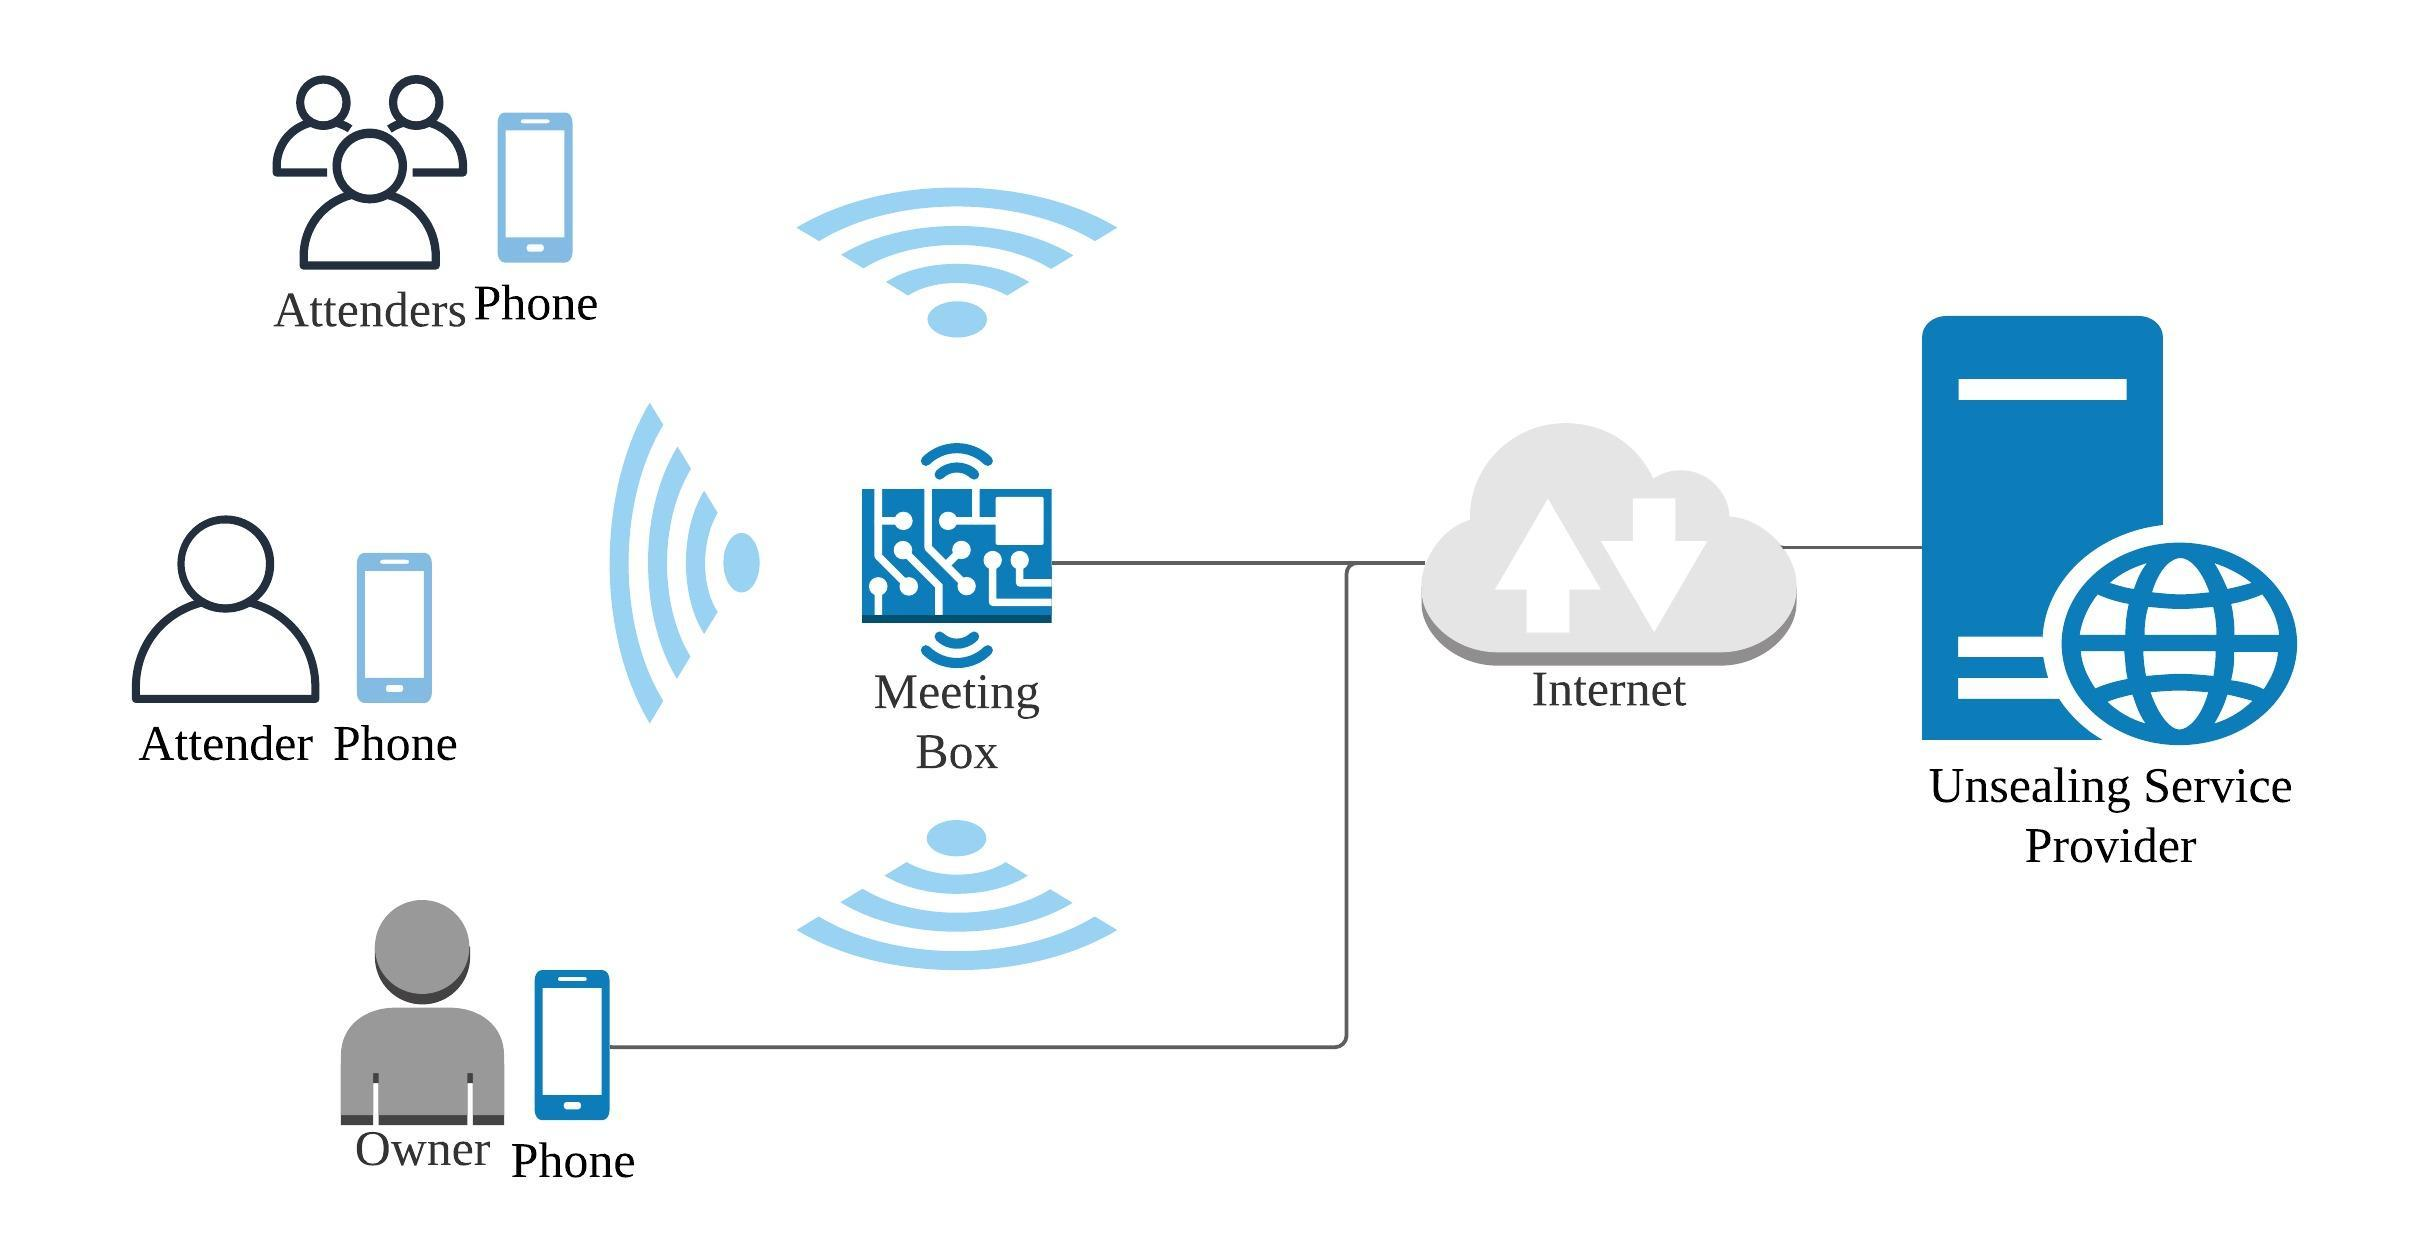
\includegraphics[width=0.9\textwidth]{single-owner-architecture}
    \caption{單一會談主持者情境圖}
    \label{fig:s-o-arch}
\end{figure}

    本系統由會談終端(MeetingBox)、會談參與者(Attender)以解封伺服器(Unsealing Service Provider)所組成。
各會談({\it Meeting Session})的會談參與者僅定義於當次會談,每次參與會談的會談參與者可為不同群體。
會談參與者於會談終端的周圍進行會談,如圖 \ref{fig:s-o-arch}。
會談終端於會談進行間開啟超音波麥克風干擾器,因此鄰近的麥克風或周邊的聲音記錄裝置,
都將因受到其干擾而失效,會談參與者無法自行有效記錄會談的聲音內容。

    會談終端於會談進行中持續紀錄聲音,內容為受到超音波麥克風干擾器干擾的會談錄音 (\DEFrecJ)。
於會談結束後,受干擾的會談聲音記錄 (\DEFrecJ),
將透過系統機制「解封會談錄音」({\it Unsealing Session Record}),
使會談參與者中的會談主持者(Owner),獲得前述機制所產生的有效會談聲音記錄 (\DEFrecREV)。


\subsection{會談參與者}

    會談參與者(Attender) 為一集合,代表所有當次會談 ({\it Meeting Session}) 的所有參與者。
會談參與者包含會談主持者(Owner),為會談主持者的超集合。其餘非會談主持者的會談參與者視為一般參與者。
會談參與者透過會談終端上的控制介面與其互動,進而控制會談的生命週期。

    於會談進行中,會談參與者受到會談終端中的超音波麥克風干擾器的干擾,使得隨身的麥克風或聲音記錄裝置,
都將因受到干擾而失效,無法有效記錄會談內容。例如:智慧型手機、智慧手錶、筆電、平板、智慧喇叭等。


\subsection{會談主持者}

\begin{figure}[H]
    \centering
    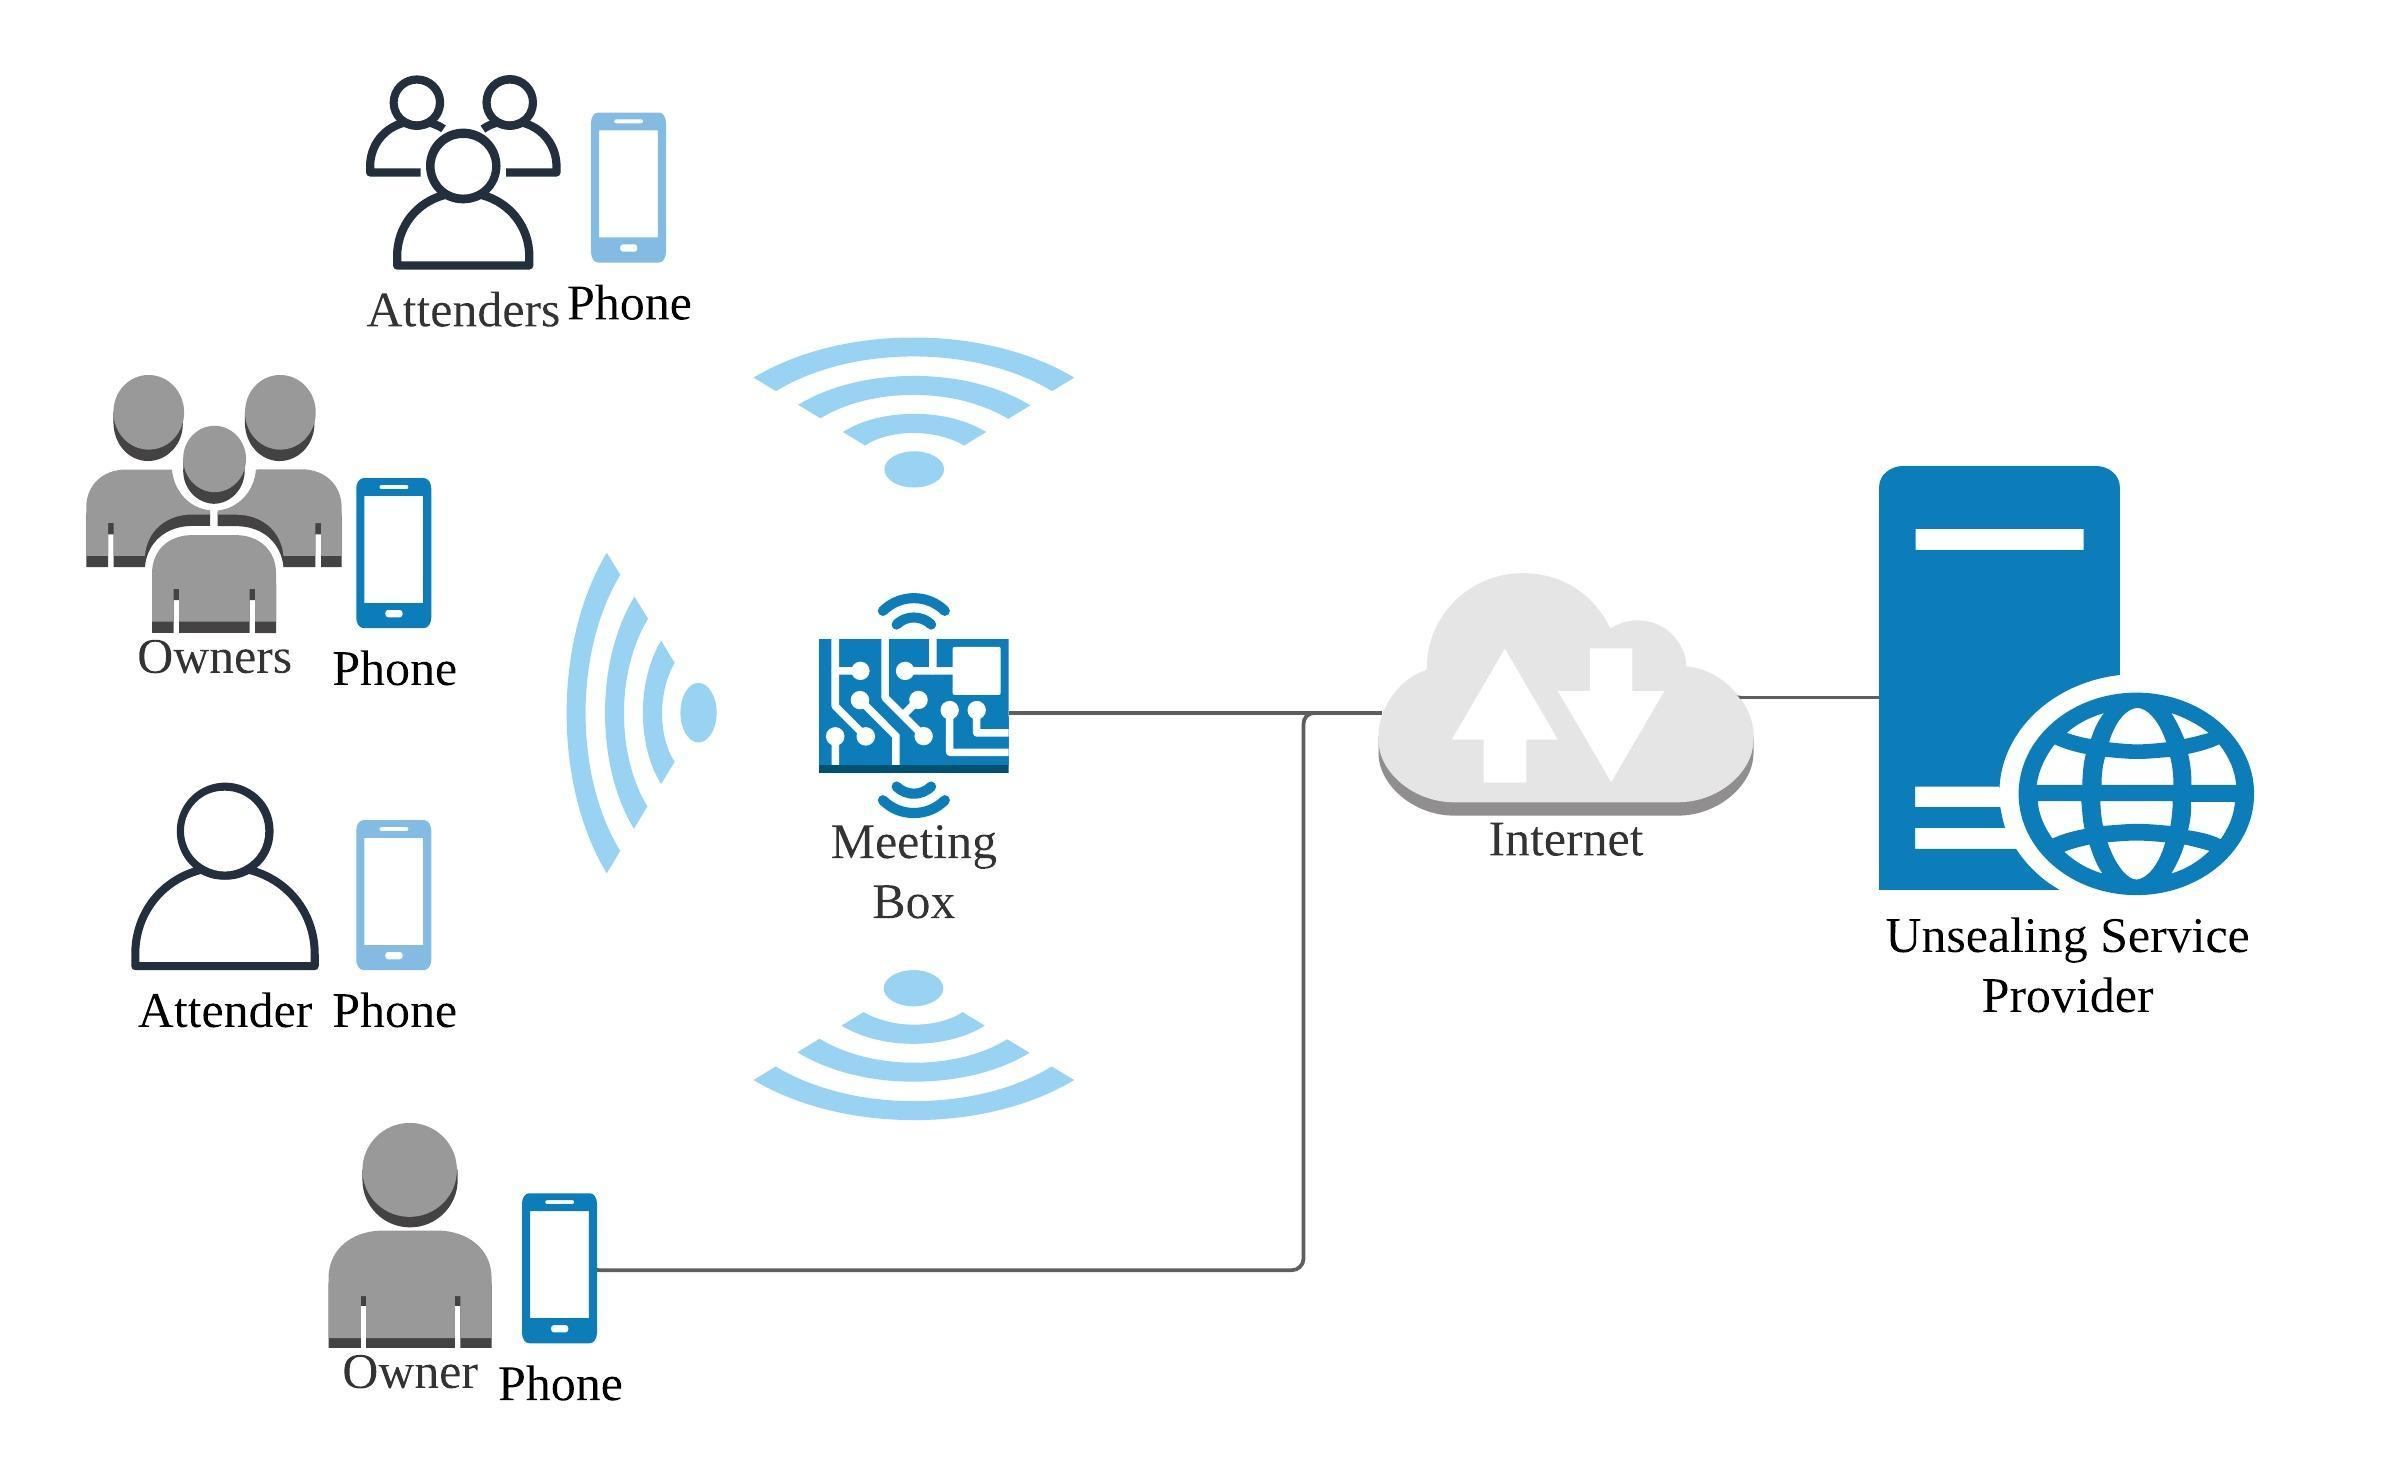
\includegraphics[width=0.9\textwidth]{multi-owner-architecture}
    \caption{多會談主持者情境圖}
    \label{fig:m-o-arch}
\end{figure}

    會談主持者(Owner),屬於會談參與者(Attender),為會談參與者的子集合,定義為會談參與者中的特權角色。
會談主持者如未執行本研究所設計的系統機制「註冊會談主持者」 (Register Owner),則視為一般參與者。
於會談 ({\it Meeting Session}) 結束後,
會談主持者有能力決定是否執行系統機制「解封會談錄音」({\it Unsealing Session Record}),
並獲取解封會談錄音後所產生的有效會談聲音記錄 (\DEFrecREV)。

    會談主持者可以是一或多人。當會談中只有一個會談主持者時,為「單一會談主持者」情境,
系統架構如圖 \ref{fig:s-o-arch}。當會談中多於一個會談主持者時,為「多會談主持者」情境,
系統架構如圖 \ref{fig:m-o-arch} 所示。

    會談主持者持有智慧型裝置,且透過 App 與會談終端互動,獲取會談終端上的資訊。
並同樣有能力於會談進行中、談結束後,與解封伺服器進行通訊。


\subsection{會談終端}

    會談終端(MeetingBox),定義符號為 \DEFmeetingbox 。
會談終端部署於會談 ({\it Meeting Session}) 的場域,與會談參與者(Attender)實體接觸,
透過與會談參與者的互動,成為觸發會談生命週期改變事件的控制核心,同時也作為系統聲音紀錄的輸入來源。
故一組會談終端僅能同時間處理一場會談的進行。

    會談終端包含多個組件,如下所列:

    \begin{enumerate}
        \item 超音波麥克風干擾器:\\
            使用偽隨機數產生器 \DEFfuncPRNG{} 產生亂數頻率的超音波,於會談進行中開啟。
            用於干擾鄰近周圍含有麥克風的裝置,使其無法有效記錄會談內容。
            \DEFfuncPRNG{} 的輸入為亂數種子 \DEFseed。

        \item 錄音麥克風:\\
            用於錄製受超音波麥克風干擾器干擾的會談對話聲音記錄 (\DEFrecJ),
            與產生純超音波麥克風干擾器於麥克風的響應輸出(噪音)之聲音記錄 (\DEFrecN)。

        \item 物理控制介面:\\
            提供會談參與者操作與會談終端互動,獲得外部觸發事件。

        \item 人機互動介面:\\
            用於傳遞會談的元資料與系統狀態提示給會談參與者。

        \item 運算控制核心與網路介面:\\
            周邊裝置控制與邏輯運算核心,用於處理聲音記錄、執行加密與解封伺服器通訊等運算工作。
    \end{enumerate}


\subsection{解封伺服器}

    解封伺服器(Unsealing Service Provider),定義符號為 \DEFserver。
解封伺服器可部署於雲端,不需實體與會談參與者(Attender)接觸。
透過會談主持者(Owner)向解封伺服器註冊與授權實現存取控制,目標為取得產生效之會談聲音記錄 \DEFrecREV。
解封伺服器之設計能與多個會談終端(MeetingBox)配合,同時間處理一場以上的會談 ({\it Meeting Session}) 的進行。


\section{系統流程}
\label{sec:system-flow}

\begin{figure}[H]
    \centering
    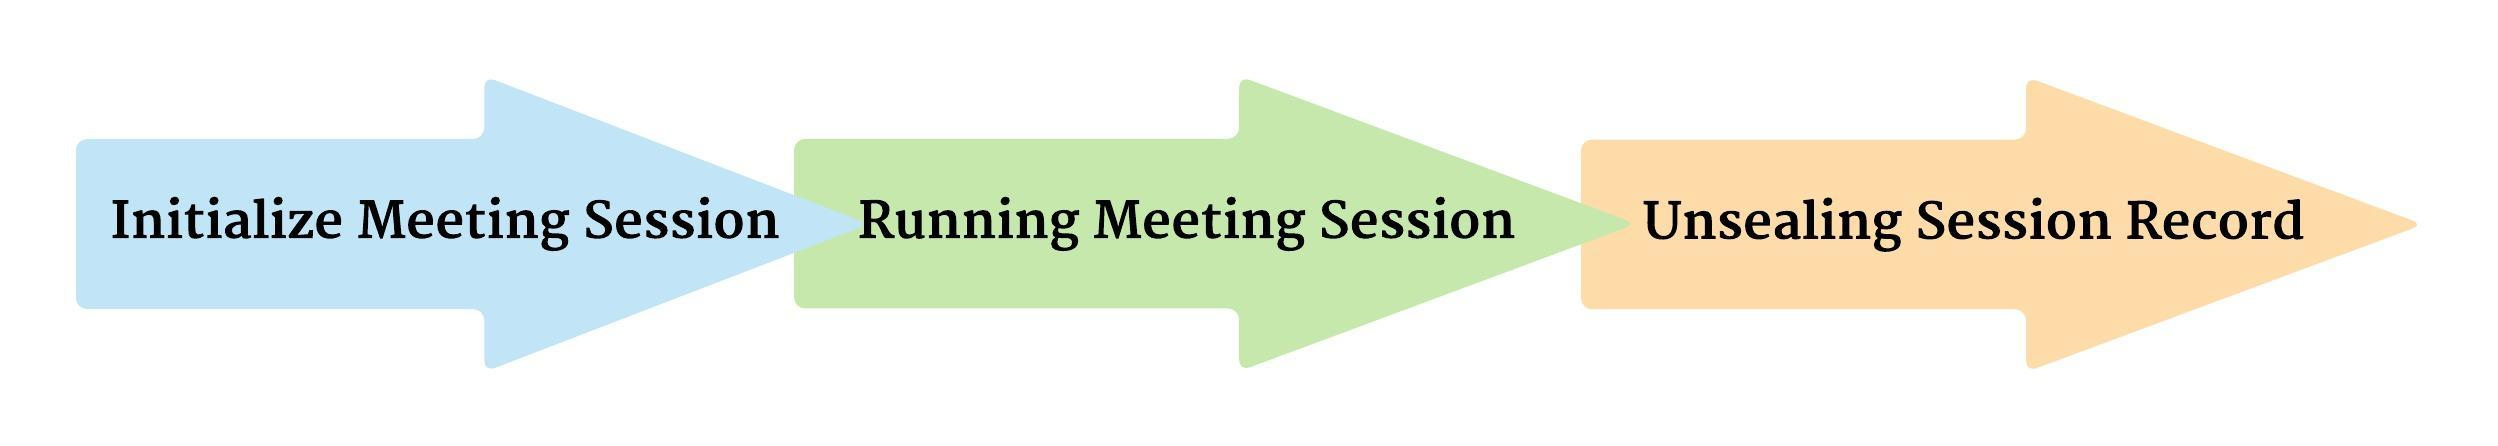
\includegraphics[width=0.9\textwidth]{system-stage}
    \caption{會談生命週期}
    \label{fig:system-stage}
\end{figure}

    本研究所設計之系統,其流程跟隨會談 ({\it Meeting Session}) 的生命週期,其分為三個階段定義。分別為:
一、「初始化會談 (Initialize {\it Meeting Session})」;二、「進行會談 (Running {\it Meeting Session})」;
三、「「解封會談錄音」({\it Unsealing Session Record})」;如圖 \ref{fig:system-stage}。

    本章節將介召會談生命週期各階段的流程步驟。
第一階段為會談的起始點,各階段依序執行,於第三階段結束,完成一次系統生命週期的循環。
透過解封伺服器與多個會談終端配合,系統可以同時存在多個會談生命週期,彼此互不干擾,獨立執行。
依據會談主持者的數量,將分為兩種情境說明討論:
一、「單一會談主持者情境 ({\it Single Owner Meeting Session})」;
二、「多會談主持者情境 ({\it Multi Owner Meeting Session})」;
當會談參與者裡僅有一位會談主持者,為單一會談主持者情境,若會談中多於一個會談主持者時,則為多會談主持者情境。

    會談終端(MeetingBox) 於談生命週期開始之前,會預先設定時間長度為 \DEFtimeMAX 的噪音 \DEFrecN,
於會談第二階段進行會談中所紀錄的聲音內容之長度,須小於  \DEFtimeMAX。
此噪音 \DEFrecN 為純超音波麥克風干擾器於麥克風的響應輸出,產生方法為選定一隨機種子 \DEFseed 作為參數,
輸入並開啟超音波麥克風干擾器,透過麥克風錄製產生。
於每次會談生命週期結束後,重複此步驟重新選定 \DEFseed 與產生 \DEFrecN。

    接續章節將說明,於單一會談主持者情境中的流程與步驟。


\subsection{初始化會談}
\label{subsec:initialize}

    此章節將說明 {\it Single Owner Meeting Session} 情境中,
{\it Meeting Session} 生命週期第一個階段:Initialize {\it Meeting Session} 的系統流程。
如圖 \ref{fig:s-o-init} 所示。

\begin{figure}[H]
    \centering
    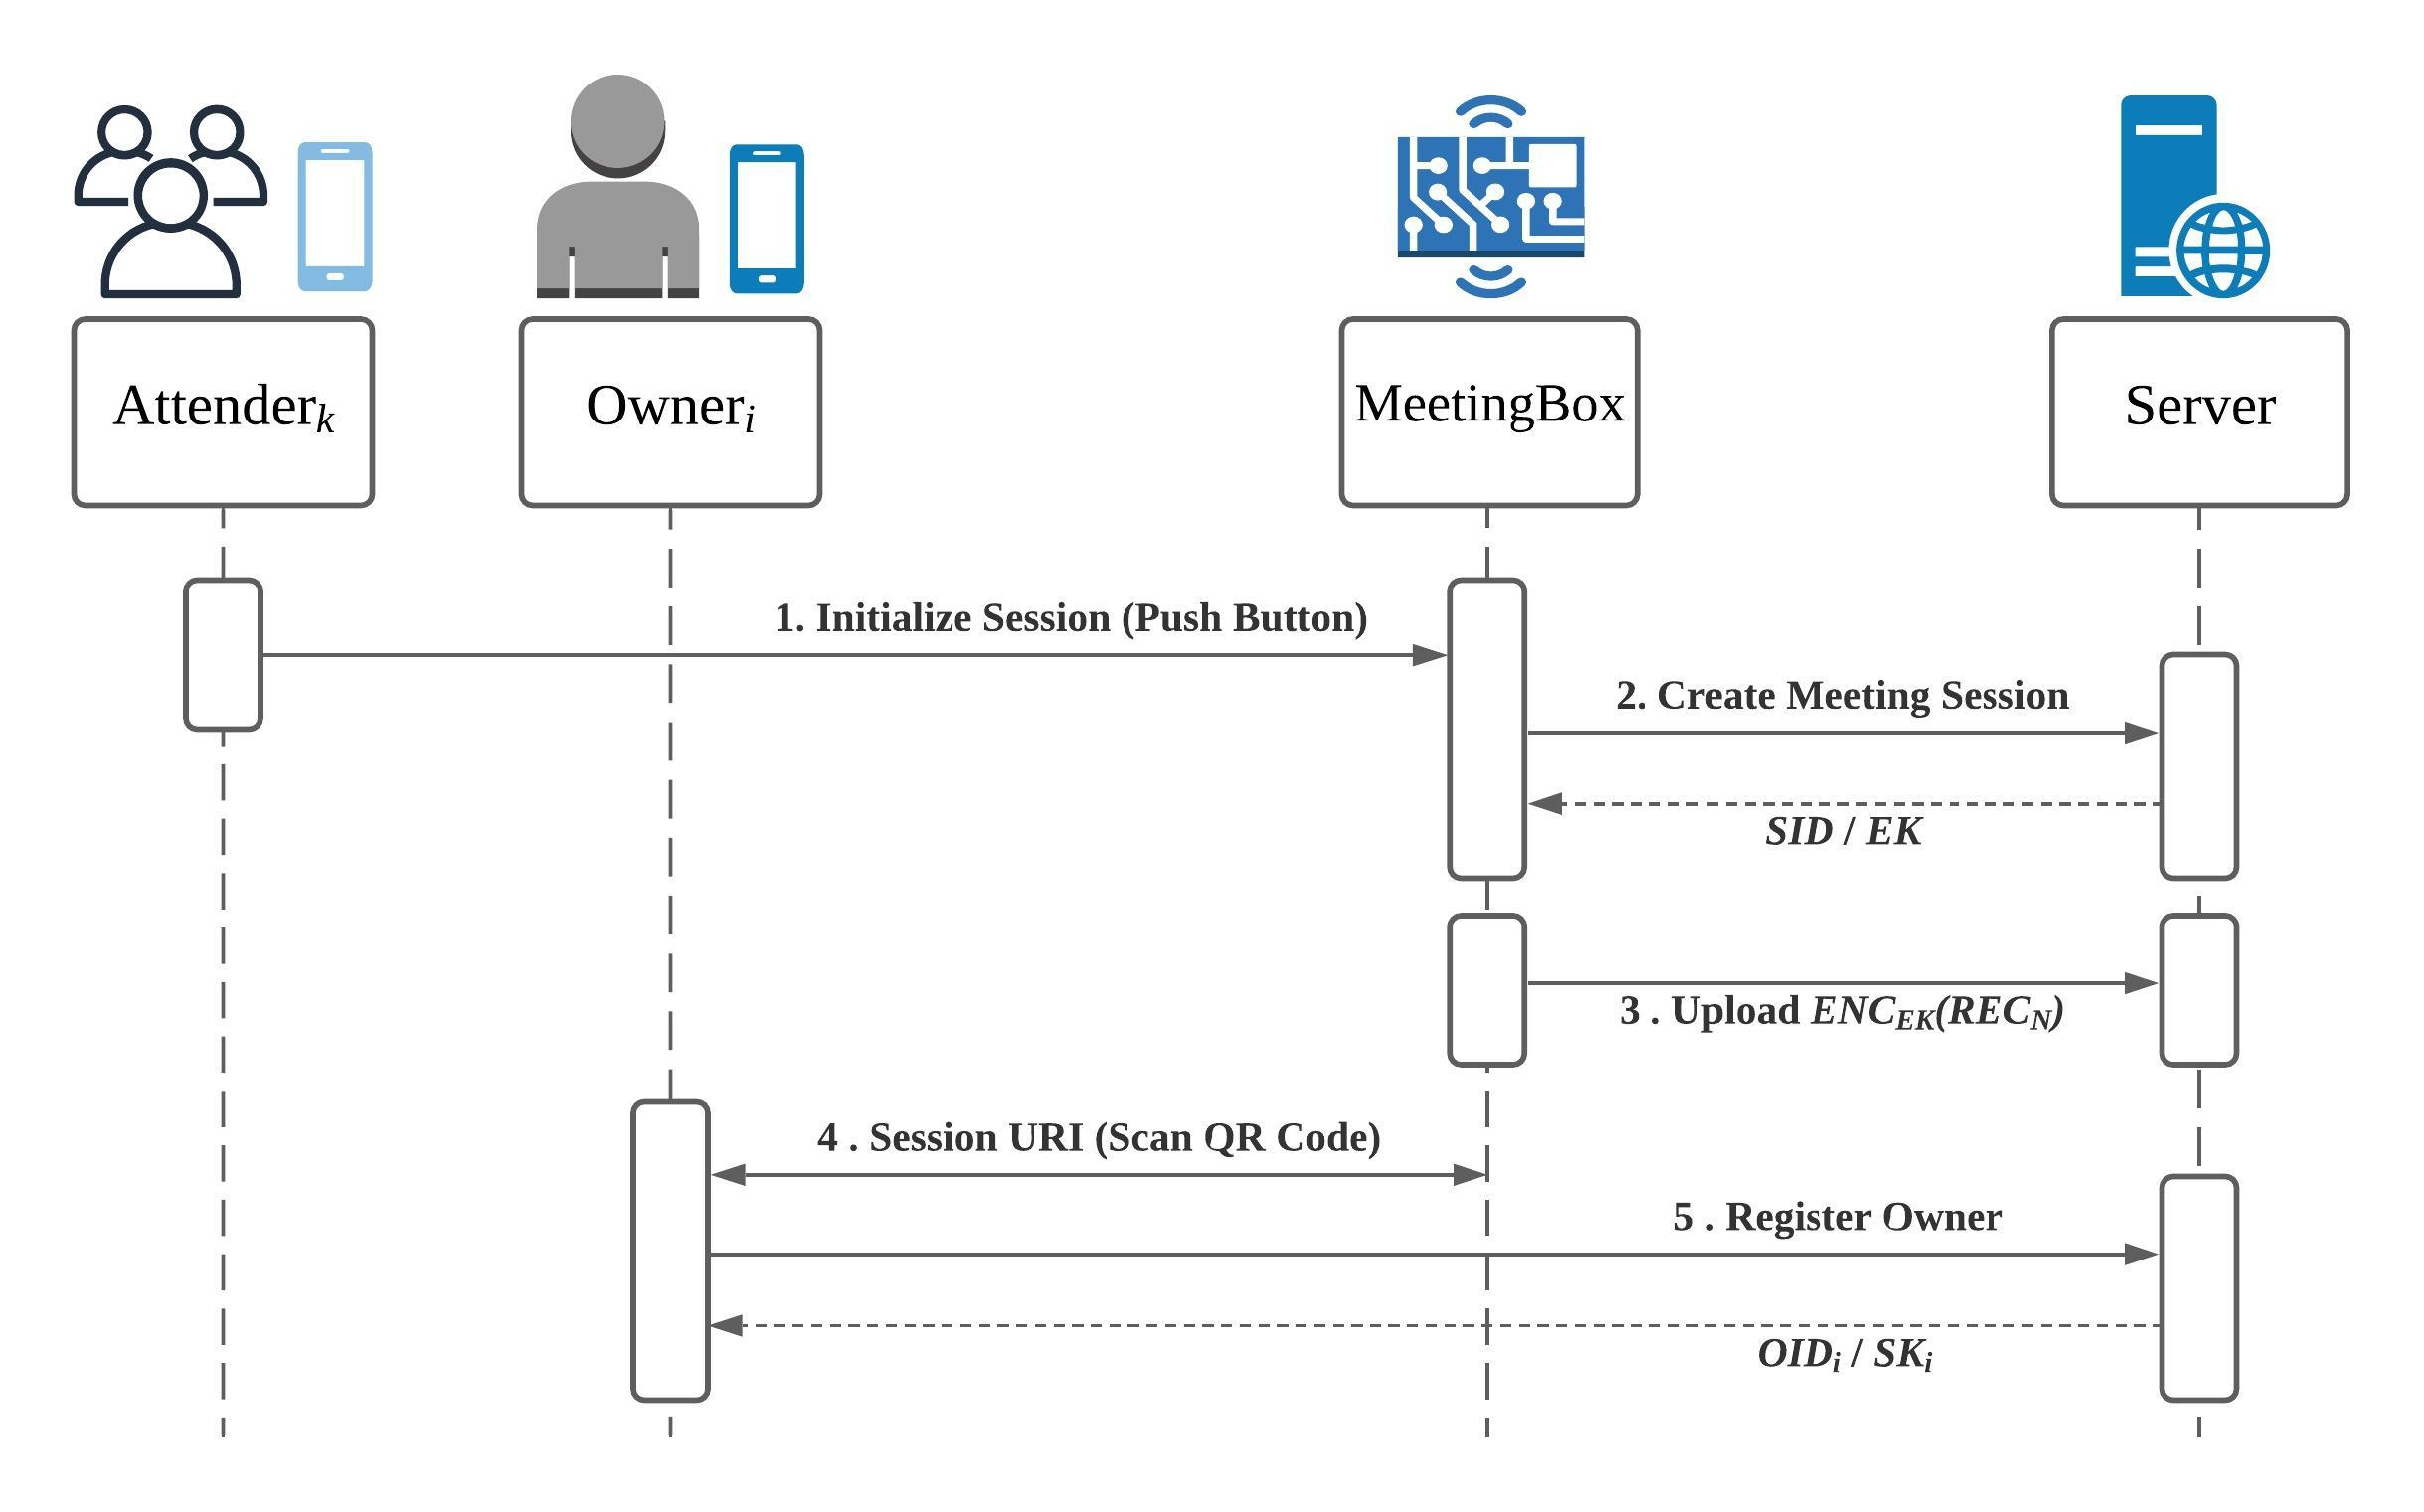
\includegraphics[width=0.9\textwidth]{single-owner-sequence-diagram-init}
    \caption{Single Owner Initialize {\it Meeting Session}}
    \label{fig:s-o-init}
\end{figure}

\begin{steps}
    \item Initialize Session (Push Button):

            Attender 在欲進行會談 MeetingBox 的周圍準備開始會談,\DEFattender 透過 MeetingBox 的物理控制介面,
        使 MeetingBox 獲得外部事件,觸發 Initialize Session。本研究實驗以按鈕為例,
        當 \DEFattender 按下 MeetingBox 上的按鈕後,觸發 MeetingBox 執行 Initialize Session。

    \item Create Meeting Session:

            MeetingBox 觸發 Initialize Session 後,首先對 Server 傳送請求 Create Meeting Session。
        Server 收到請求後產生 (\DEFsessionID, \DEFunsealKey) 並回傳至 MeetingBox。

            其中 \DEFsessionID 為此次 {\it Meeting Session} 的唯一識別碼;\DEFunsealKey 是對稱式加密金鑰,
        定義為此次 {\it Meeting Session} 的解封金鑰 (Unsealing Key)。
        \DEFsessionID 的產生必須滿足唯一性,隨機性,不可預測性,本研究實作 \DEFsessionID 以 UUID v4 為例。
        \DEFunsealKey 為對稱式加密的金鑰,其產生方式,本研究所設計之系統以 AES CFB mode 為例。

    \item Upload Encrypted \DEFrecN:

            MeetingBox 收到產生自 Server 的回傳訊息 (\DEFsessionID, \DEFunsealKey)後,使用對稱式加密演算法與金鑰 \DEFunsealKey 加密 \DEFrecN,
        在將加密後的 \DEFrecN 上傳至 Server,並銷毀於 MeetingBox 中的 \DEFunsealKey。

            前述對稱式密鑰演算法,本研究所設計之系統以 AES CFB mode 為例。本文中定義為 \DEFfuncEncEK,
        其輸入為欲加密明文資料,輸出為已加密的密文。

    \item Get Session URI (Scan QR Code):

            MeetingBox 收到產生自 Server 的回傳訊息 (\DEFsessionID, \DEFunsealKey)後,
        將 \DEFsessionID 資訊封裝為此次 {\it Meeting Session} 專用的 URI (Uniform Resource Identifier),
        並傳送給 Owner。URI 的封裝方法為,將 \DEFsessionID 填入系統已知包含 Server 網址的字串。

            前述 MeetingBox 將資訊傳遞給 Owner 的方法,本研究以 MeetingBox 搭配螢幕顯示 QR Code 為例。
        \DEFowner 持智慧裝置,掃描 MeetingBox 螢幕顯示的 QR Code,以獲得 \DEFsessionID 封裝後的 URI 。

    \item Register Owner:

            \DEFowner 收到 MeetingBox 產生的 URI 後,
        使用此 URI 向 Server 進行系統機制「註冊會談主持者」 (Register Owner)。運作細節如下:
        一、\DEFowner 對 Server 發送 Register Owner 請求;
        二、Server 收到 Register Owner 請求後,隨即產生一組公私金鑰對 (\DEFpublicKey, \DEFprivateKey)
        與 \DEFowner 的唯一識別碼 \DEFownerID,
        並將請求來源 URI 中的 \DEFsessionID 與公開金鑰 \DEFpublicKey 和 \DEFownerID 做關聯綁定;
        三、回傳私密金鑰 \DEFprivateKey 與 \DEFownerID 給 \DEFowner,且銷毀於 Server 中的\DEFprivateKey;

            在 {\it Single Owner Meeting Session} 情境中,只存在一個 Owner,
        因此當唯一 Owner 執行成功後,即完成此系統步驟,進入下一階段。
        Onwer 為 Attender 中的特權角色,其特權來源為 \DEFowner 的 \DEFprivateKey,
        因此 Owner 須妥善保管 \DEFprivateKey,維持其機密性。

            \DEFownerID 的產生必須滿足唯一性,隨機性,
        不可預測性,本研究實作 \DEFownerID 以 UUID v4 為例。
        前述公私金鑰對的產生方法,本研究所設計之系統以 RSA PKCS \#1 為例。
\end{steps}

\subsection{進行會談}
\label{subsec:sessioning}

    此章節將說明 {\it Single Owner Meeting Session} 情境中,
{\it Meeting Session} 生命週期第二個階段:Running {\it Meeting Session} 的系統流程。
如圖 \ref{fig:s-o-sessioning} 所示。

\begin{figure}[H]
    \centering
    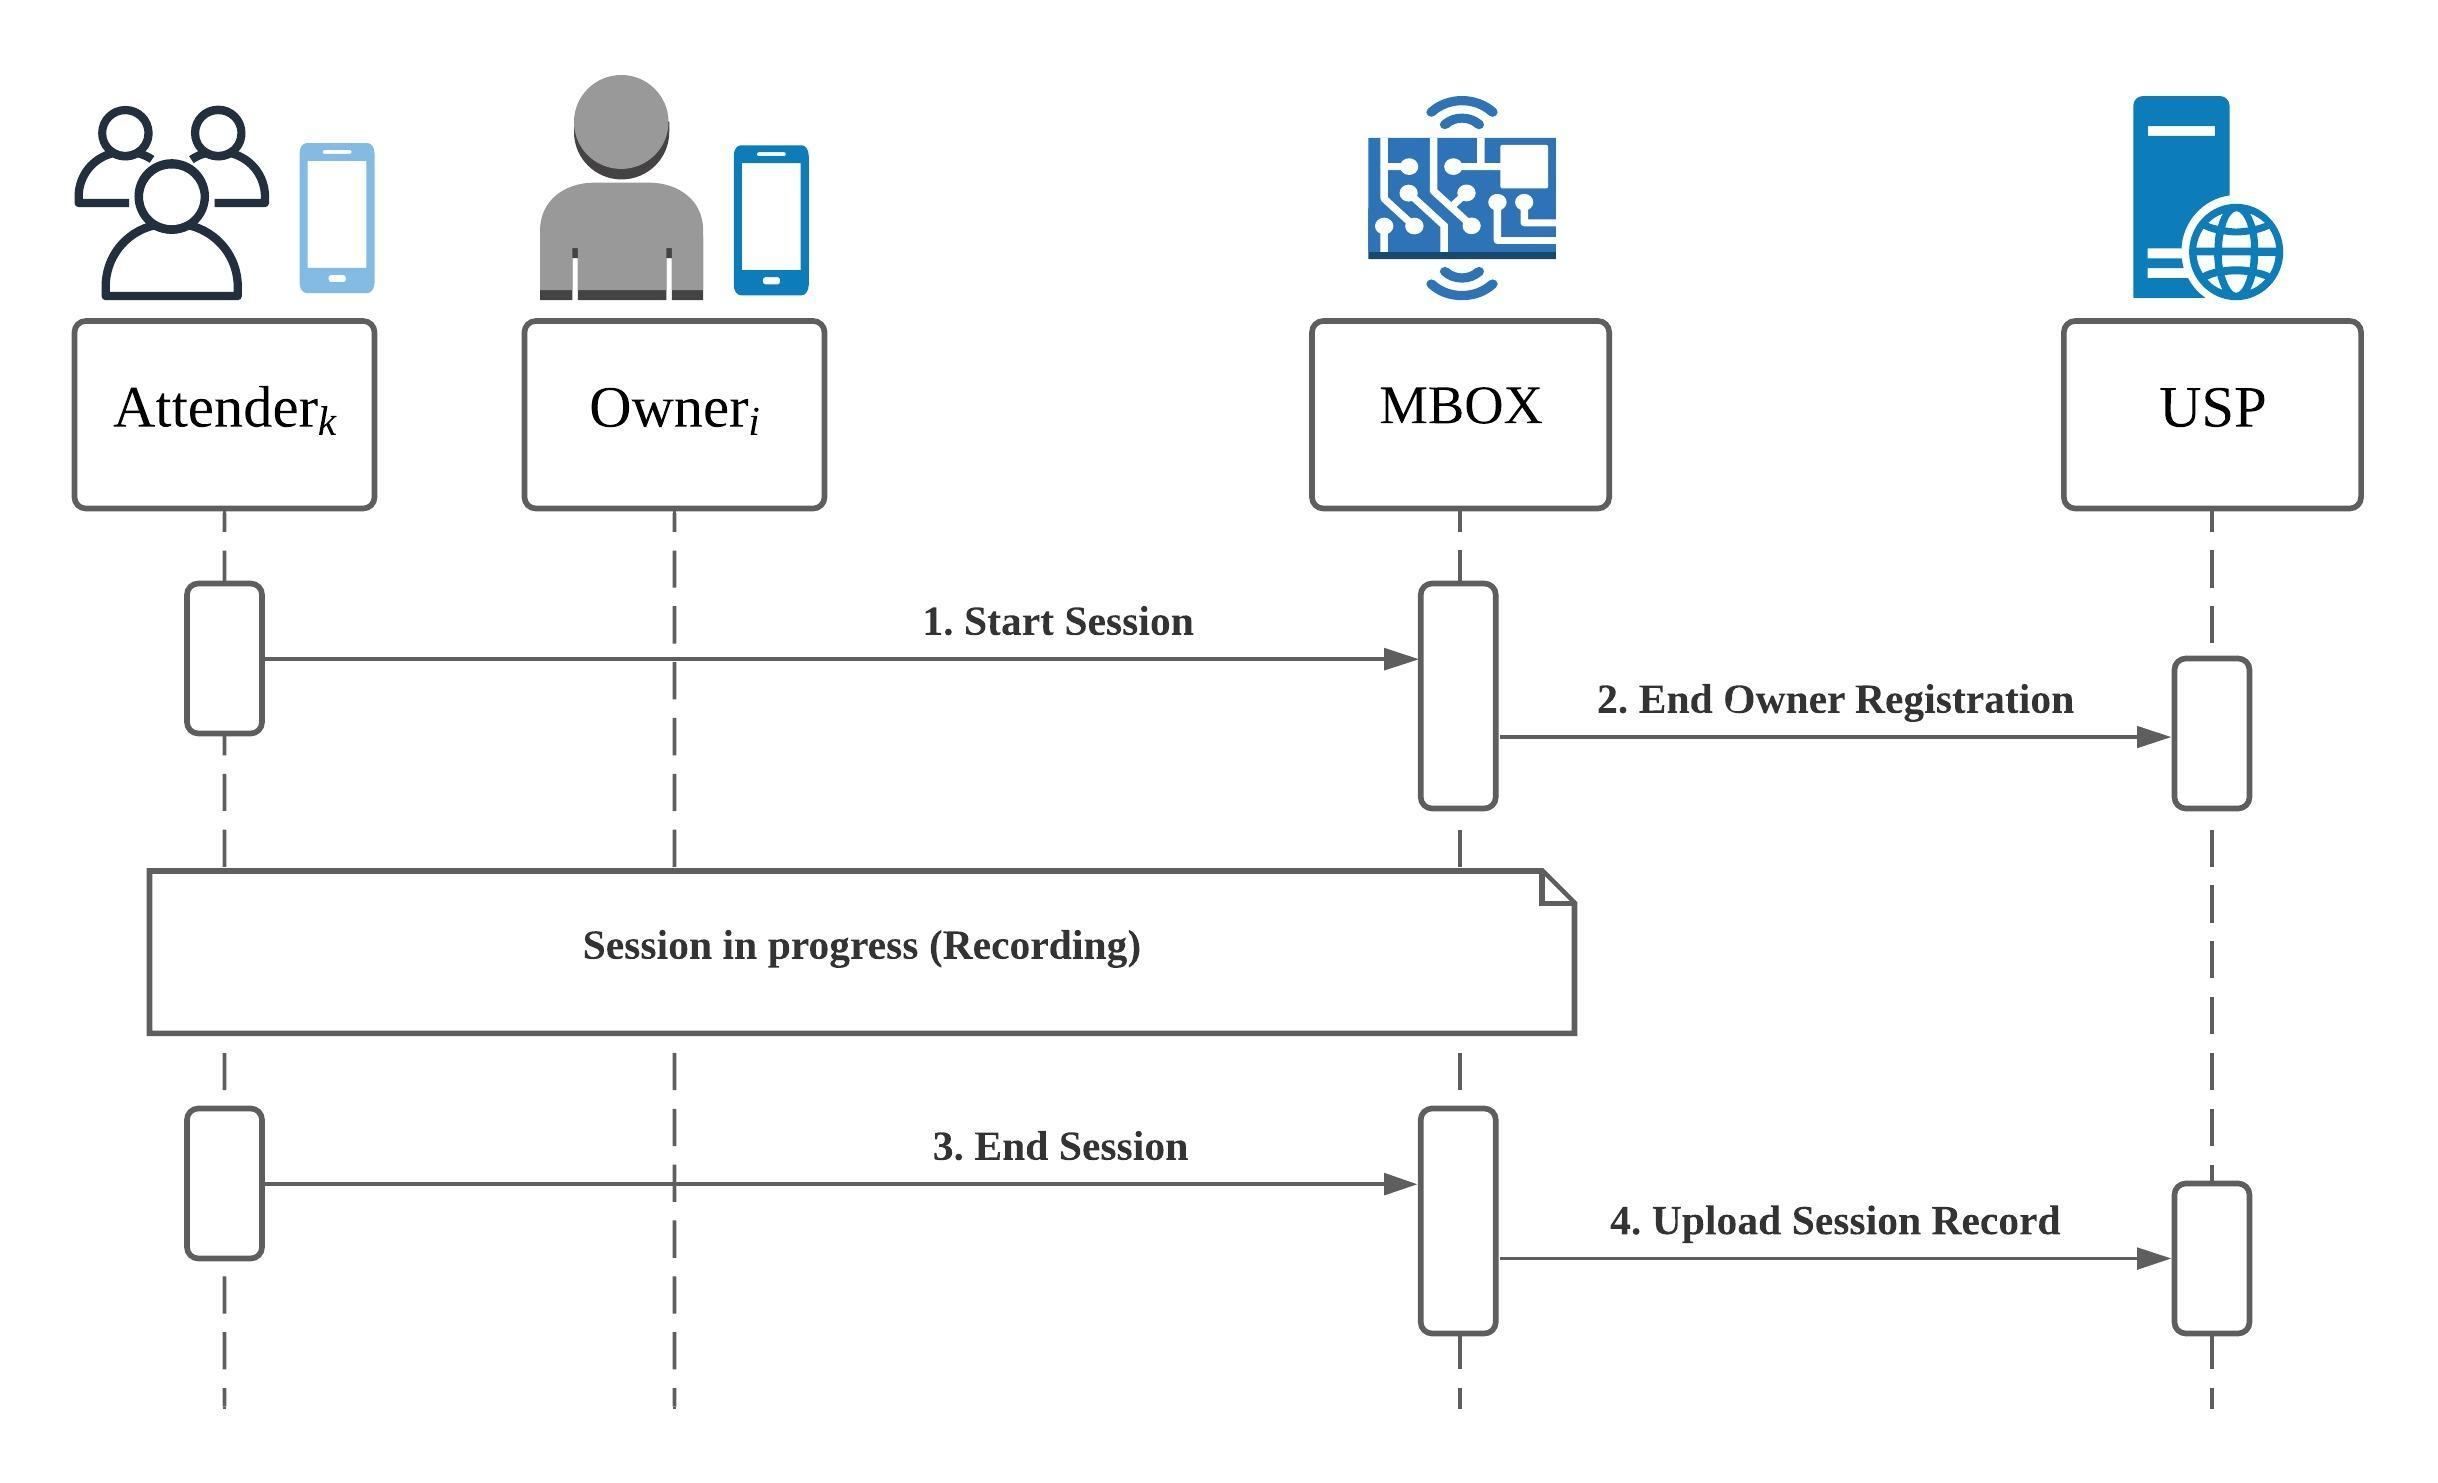
\includegraphics[width=0.9\textwidth]{single-owner-sequence-diagram-sessioning}
    \caption{Single Owner Running {\it Meeting Session}}
    \label{fig:s-o-sessioning}
\end{figure}

\begin{steps}
    \item Start Session (Push Button):

            進入到此階段代表 Owner 已經完成系統機制 Register Owner,MeetingBox 也已初始化完成。
        此時 \DEFattender 即可透過 MeetingBox 的物理控制介面,使 MeetingBox 獲得外部事件,
        觸發 Start Session。

            本研究實驗以按鈕為例,當 \DEFattender 按下 MeetingBox 上的按鈕後,
        觸發 MeetingBox 執行 Start Session。

    \item End Owner Registration:

            MeetingBox 觸發 Start Session 後,接續觸發 Server 執行 End Owner Registration,
        其運作細節如下:一、MeetingBox 對 Server 傳送 End Owner Registration 請求;
        二、Server 透過限制無法在同 \DEFsessionID 綁定新的\DEFprivateKey,
        來終止此 {\it Meeting Session} 註冊產生新的 Owner;
        三、透過 \DEFunsealKey 派生出 \DEFowner 的代理金鑰,定義為 \DEFagentKey。當 \DEFagentKey 產生完即銷毀 \DEFunsealKey 。
        在 {\it Single Owner Meeting Session} 情境中,\DEFagentKey 的值即等於 \DEFunsealKey。
        四、Server 使用此情境中唯一 \DEFowner 的公開金鑰 \DEFpublicKey,透過非對稱式金鑰演算法加密將 \DEFagentKey 加密,
        並銷毀 \DEFagentKey;Server 即完成此系統步驟。

            前述非對稱式金鑰加密演算法,本研究所設計之系統 RSA PKCS \#1 為例。 本文中定義為 \DEFfuncEncPK,
        其輸入為欲加密明文資料,輸出為已加密的密文。加密後的 \DEFagentKey 定義為 \DEFowner 的 \DEFakEnc,
        待 \DEFowner 將其解密方可還原 \DEFagentKey。
        意即,在此情境中,唯一 \DEFowner 的 \DEFakEnc 即為透過 \DEFfuncEncPK 加密的 \DEFunsealKey。

            隨後 MeetingBox 開啟麥克風與超音波麥克風干擾器,並透過 MeetingBox 上的人機互動介面提示系統已經開始錄音。
        麥克風錄製的聲音內容結果 \DEFrecJ,此為超音波麥克風干擾器與會談聲音內容的疊加,屬非有效之聲音記錄。
        此時 Attender 即可進行私密會談,不用擔心有其他麥克風或聲音記錄裝置可以取得有效之聲音記錄。
        前述人機互動介面,本研究實驗以錄音指示燈與螢幕為例,當開始錄音時,將會提示當下系統狀態。

    \item End Session (Push Button):
ㄑ
            當會談對話結束時時 \DEFattender 即可透過 MeetingBox 的物理控制介面,使 MeetingBox 獲得外部事件,
        觸發 End Session。MeetingBox 在此時會關閉麥克風與超音波麥克風干擾器,並產生 \DEFrecJ。
        MeetingBox 上的人機互動介面同時提示系統已結束錄音。

            本研究實驗以按鈕為例,當 \DEFattender 再次按下 MeetingBox 上的按鈕後,
        觸發 MeetingBox 執行 End Session。人機互動介面則以錄音指示燈與螢幕為例,
        當錄音已結束時,前述兩者人機互動介面將會提示當下系統狀態為 End Session。

    \item Upload \DEFrecJ:

            當 Attender 透過 MeetingBox 上的物理控制介面觸發 End Session 後,
        接續觸發 MeetingBox 值行此步驟。此時 MeetingBox 將 End Seesion 步驟結束所產生的 \DEFrecJ,
        上傳至 Server。上傳成功後,即完成進入下一階段。
\end{steps}


\subsection{解封會談錄音}
\label{subsec:unseal}

    此章節將說明 {\it Single Owner Meeting Session} 情境中,
{\it Meeting Session} 生命週期第三個階段:{\it Unseal} 的系統流程。
如圖 \ref{fig:s-o-unseal} 所示。此階段執行於 Running {\it Meeting Session} 之後,
Attender 間的談話已結束,Attender 可以離開會談的場域,且不再需要與 MeetingBox 實體接觸。
此階段僅 Owner 與 Server 互動,透過此階段機制,最終可取得有效之會談聲音記錄 (\DEFrecREV)。
本研究所設計之系統可以確保 Server 在 Running {\it Meeting Session}結束後,
直到成功解封 ({\it Unseal})之前,\DEFrecREV 保有機密性。

\begin{figure}[H]
    \centering
    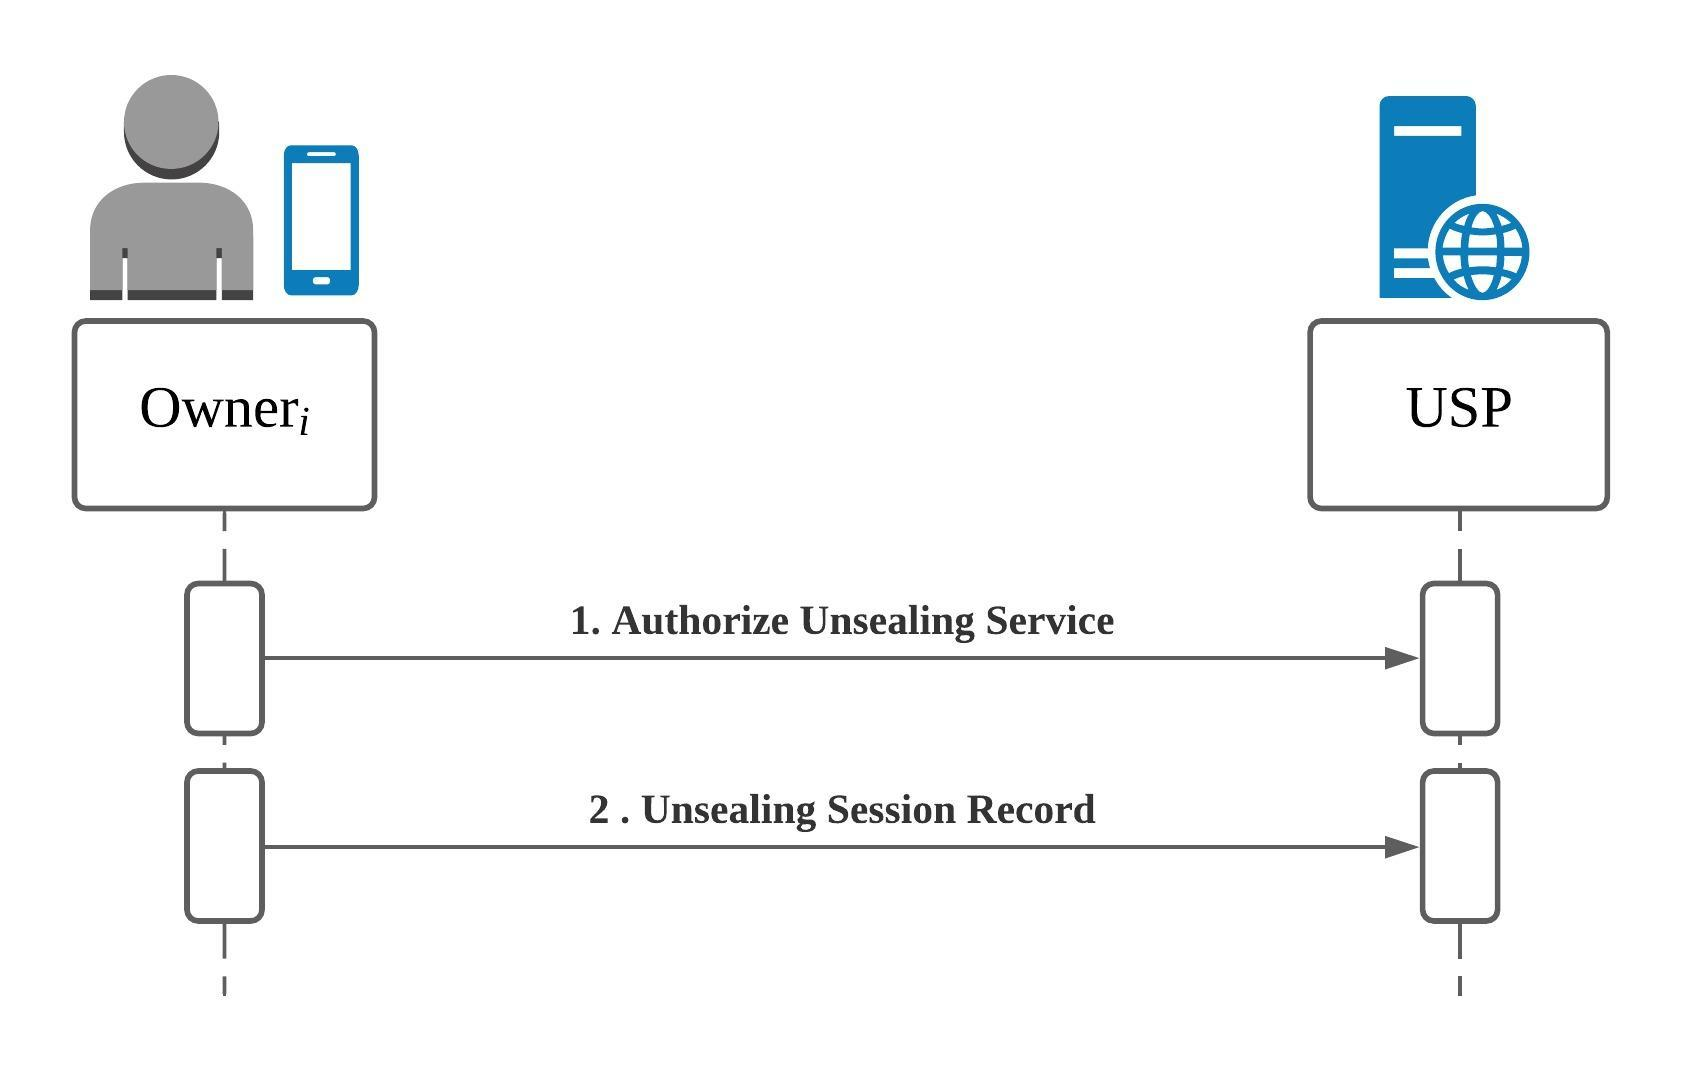
\includegraphics[width=0.7\textwidth]{single-owner-sequence-diagram-unseal}
    \caption{Single Owner {\it Unseal}}
    \label{fig:s-o-unseal}
\end{figure}

\begin{steps}
    \item Unseal Session Record Request:

            在會談對話結束後,Owner 欲取得當時的有效聲音紀錄,則執行此機制。
        \DEFowner 向 Server 傳送 Unseal Session Record Request,
        Server 則回傳 \DEFowner 的 \DEFakEnc。
        {\it Single Owner Meeting Session} 情境中,只有單一個 Owner,
        因此傳送至 \DEFowner 的 \DEFakEnc 其內容,即為使用 \DEFfuncEncPK 加密的 \DEFunsealKey。

    \item Solve Challenge:

            \DEFowner 收到 Server 回傳的 \DEFakEnc 後,因 \DEFowner 持有 \DEFprivateKey,
        因此 \DEFowner 有能力透過相同的非對稱式加密演算法透過其解密。
        而 \DEFakEnc 解密後的明文,本文將其定義為 \DEFakEncDec。

            得到 \DEFakEncDec 後,\DEFowner 再將其透過 \DEFprivateKey 使用數位簽章演算法簽名,
        所產生之簽章,本文定義為 \DEFakEncDecSig。

            \DEFowner 成功產生 \DEFakEncDec 與 \DEFakEncDecSig 後,
        將兩者作為參數向 Server 請求 Solve Challenge。
        Server 收到來自\DEFowner 的 \DEFakEncDec 與 \DEFakEncDecSig 之後,驗證 \DEFakEncDecSig 是否正確。
        透過 Server 的 \DEFpublicKey 利用數位簽章演算法驗證 \DEFakEncDecSig 是否為合法的簽章。
        若簽章合法,依據其不可否認性,Server 得以信任 \DEFakEncDec 的是產生自 \DEFowner。

            於 {\it Single Owner Meeting Session} 情境中,
        \DEFakEnc 的內容為使用 \DEFfuncEncPK 加密的 \DEFunsealKey。
        而 \DEFakEncDec 為解密後的 \DEFakEnc ,即為 \DEFunsealKey,即完成此步驟。
        前述非對稱式金鑰加密演算法,本研究所設計之系統以 RSA PKCS \#1 為例。其解密方法,
        本文定義為 \DEFfuncDecSK,輸入為 \DEFfuncEncPK 輸出的密文,輸出為 \DEFfuncEncPK 的明文輸入。

            前述數位簽章演算法,本研究以 RSA PKCS \#1 與 SHA256 為例。其簽名方法,本文定義為 \DEFfuncSignSK,
        輸入為欲簽名的資料,輸出為資料的簽章。驗證簽章方法,本文定義為 \DEFfuncVerfPK,
        輸入為欲驗證簽名的資料與簽章,輸出為合法與否。

    \item Access Session Record:

            Owner 在前一步驟 Solve Challenge 成功之後,即可再向 Server 發出 Access Session Record 請求。
        若於 Solve Challenge 成功,代表 Server 已獲得此 {\it Meeting Session} 的 \DEFunsealKey。
        此時即可將 \DEFrecN 透過 \DEFunsealKey 輸入對稱式加密演算法的解密函數還原獲得 \DEFrecN。
        前述對稱式加密演算法的解密函數,本研究以 AES CFB mode 為例。本文中定義為 \DEFfuncDecEK,
        其輸入為欲解密的密文資料,輸出解密後的明文。

            Server 上儲存的 \DEFrecJ 為非有效聲音紀錄,其原因為含有高信噪比的噪音。
        此噪音由 MeetingBox 的 超音波麥克風干擾器所產生,與 \DEFrecN 有高相似度與關聯度。
        因此透過 \DEFrecN 與 \DEFrecJ 輸入 「自適應噪音消除」(ANC),即可獲得有效會談聲音記錄。
        透過 ANC 還原的有效會談聲音記錄,本文定義為 \DEFrecREV。
\end{steps}


\subsection{{\it Multi Owner Meeting Session}}

此章節將說明 Multi Owner Meeting Session 情境中,系統生命週期階段的流程步驟。
當存在 {\it Meeting Session} 中 Owner 數量為二人以上,即定義為 Multi Owner Meeting Session 之情境。
於此情境中,{\it Meeting Session} 生命週期的三個階段與前篇 Single Owner Meeting Session 情境相似。
其差異之處在於 Owner 數量大於二人。基於前篇 Single Owner Meeting Session 情境,
僅需小幅度的系統改動與引入 Shamir's Secret Sharing,即可達成 Multi Owner Meeting Session 情境。

\begin{figure}[H]
    \centering
    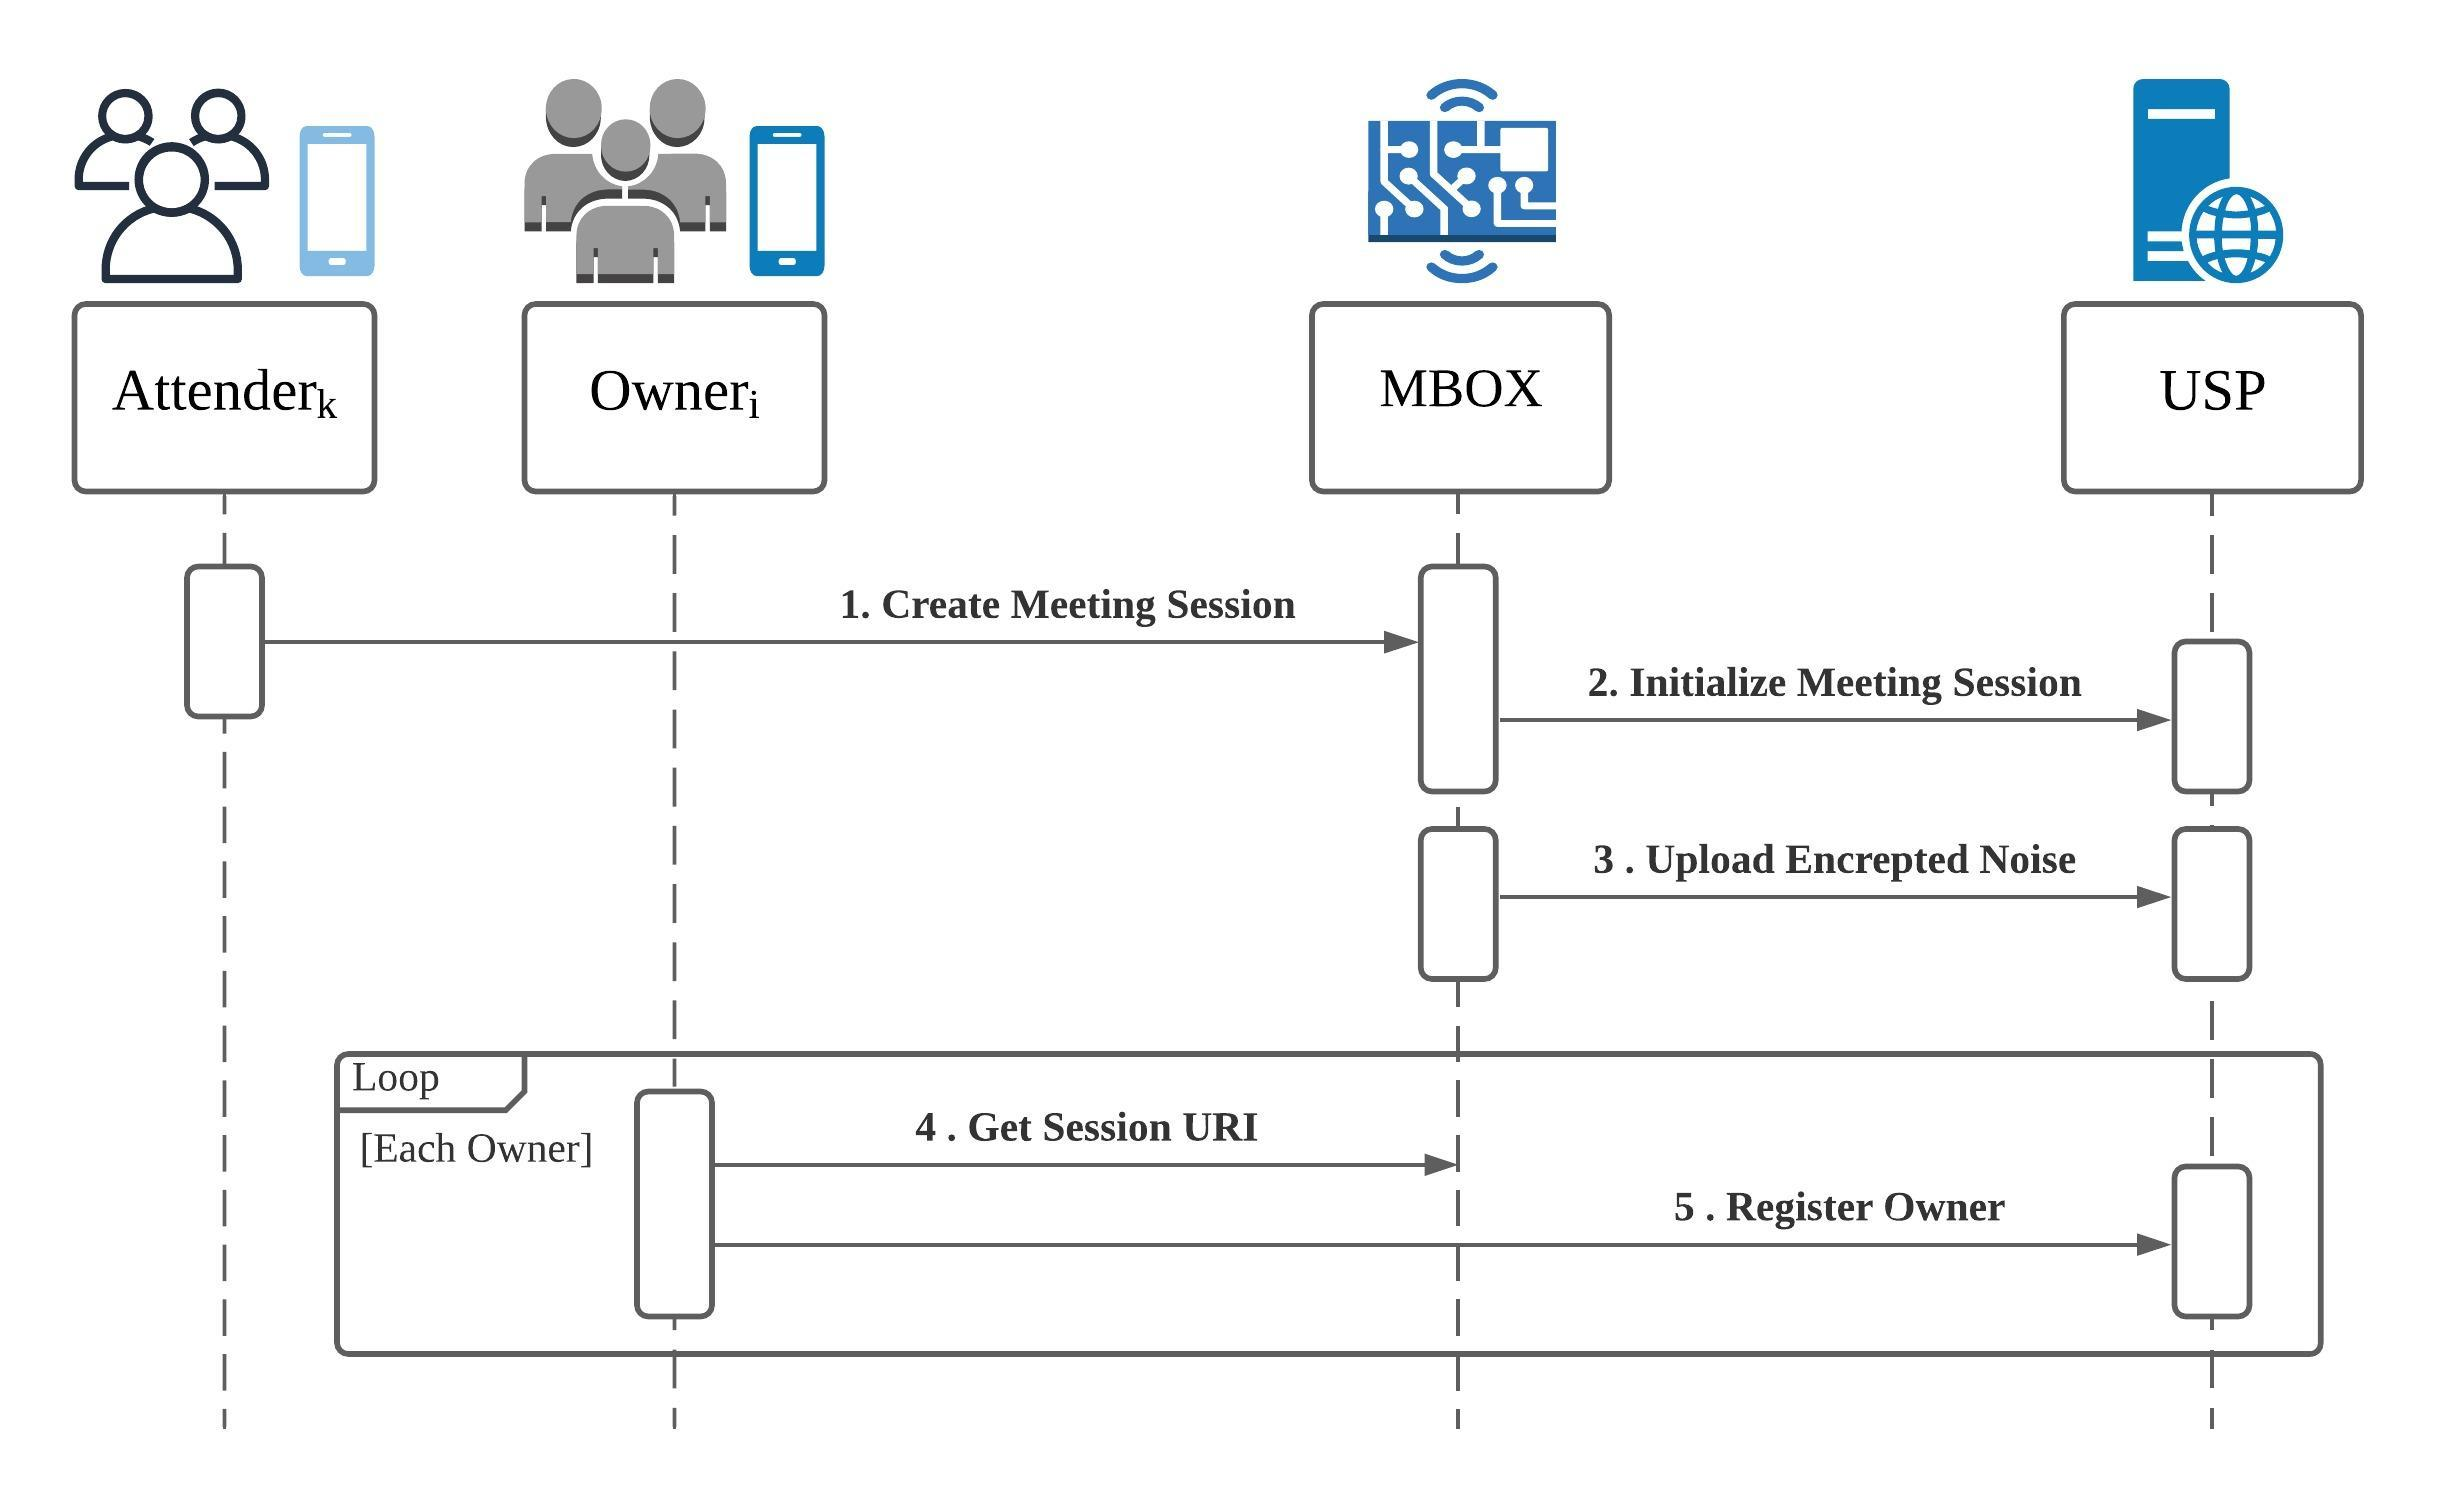
\includegraphics[width=0.9\textwidth]{multi-owner-sequence-diagram-init}
    \caption{Multi Owner Initialize {\it Meeting Session}}
    \label{fig:m-o-init}
\end{figure}

    {\it Multi Owner Meeting Session} 情境中,
{\it Meeting Session} 生命週期第一個階段:Initialize {\it Meeting Session} 的系統流程。
如圖 \ref{fig:s-o-init} 所示。

\begin{figure}[H]
    \centering
    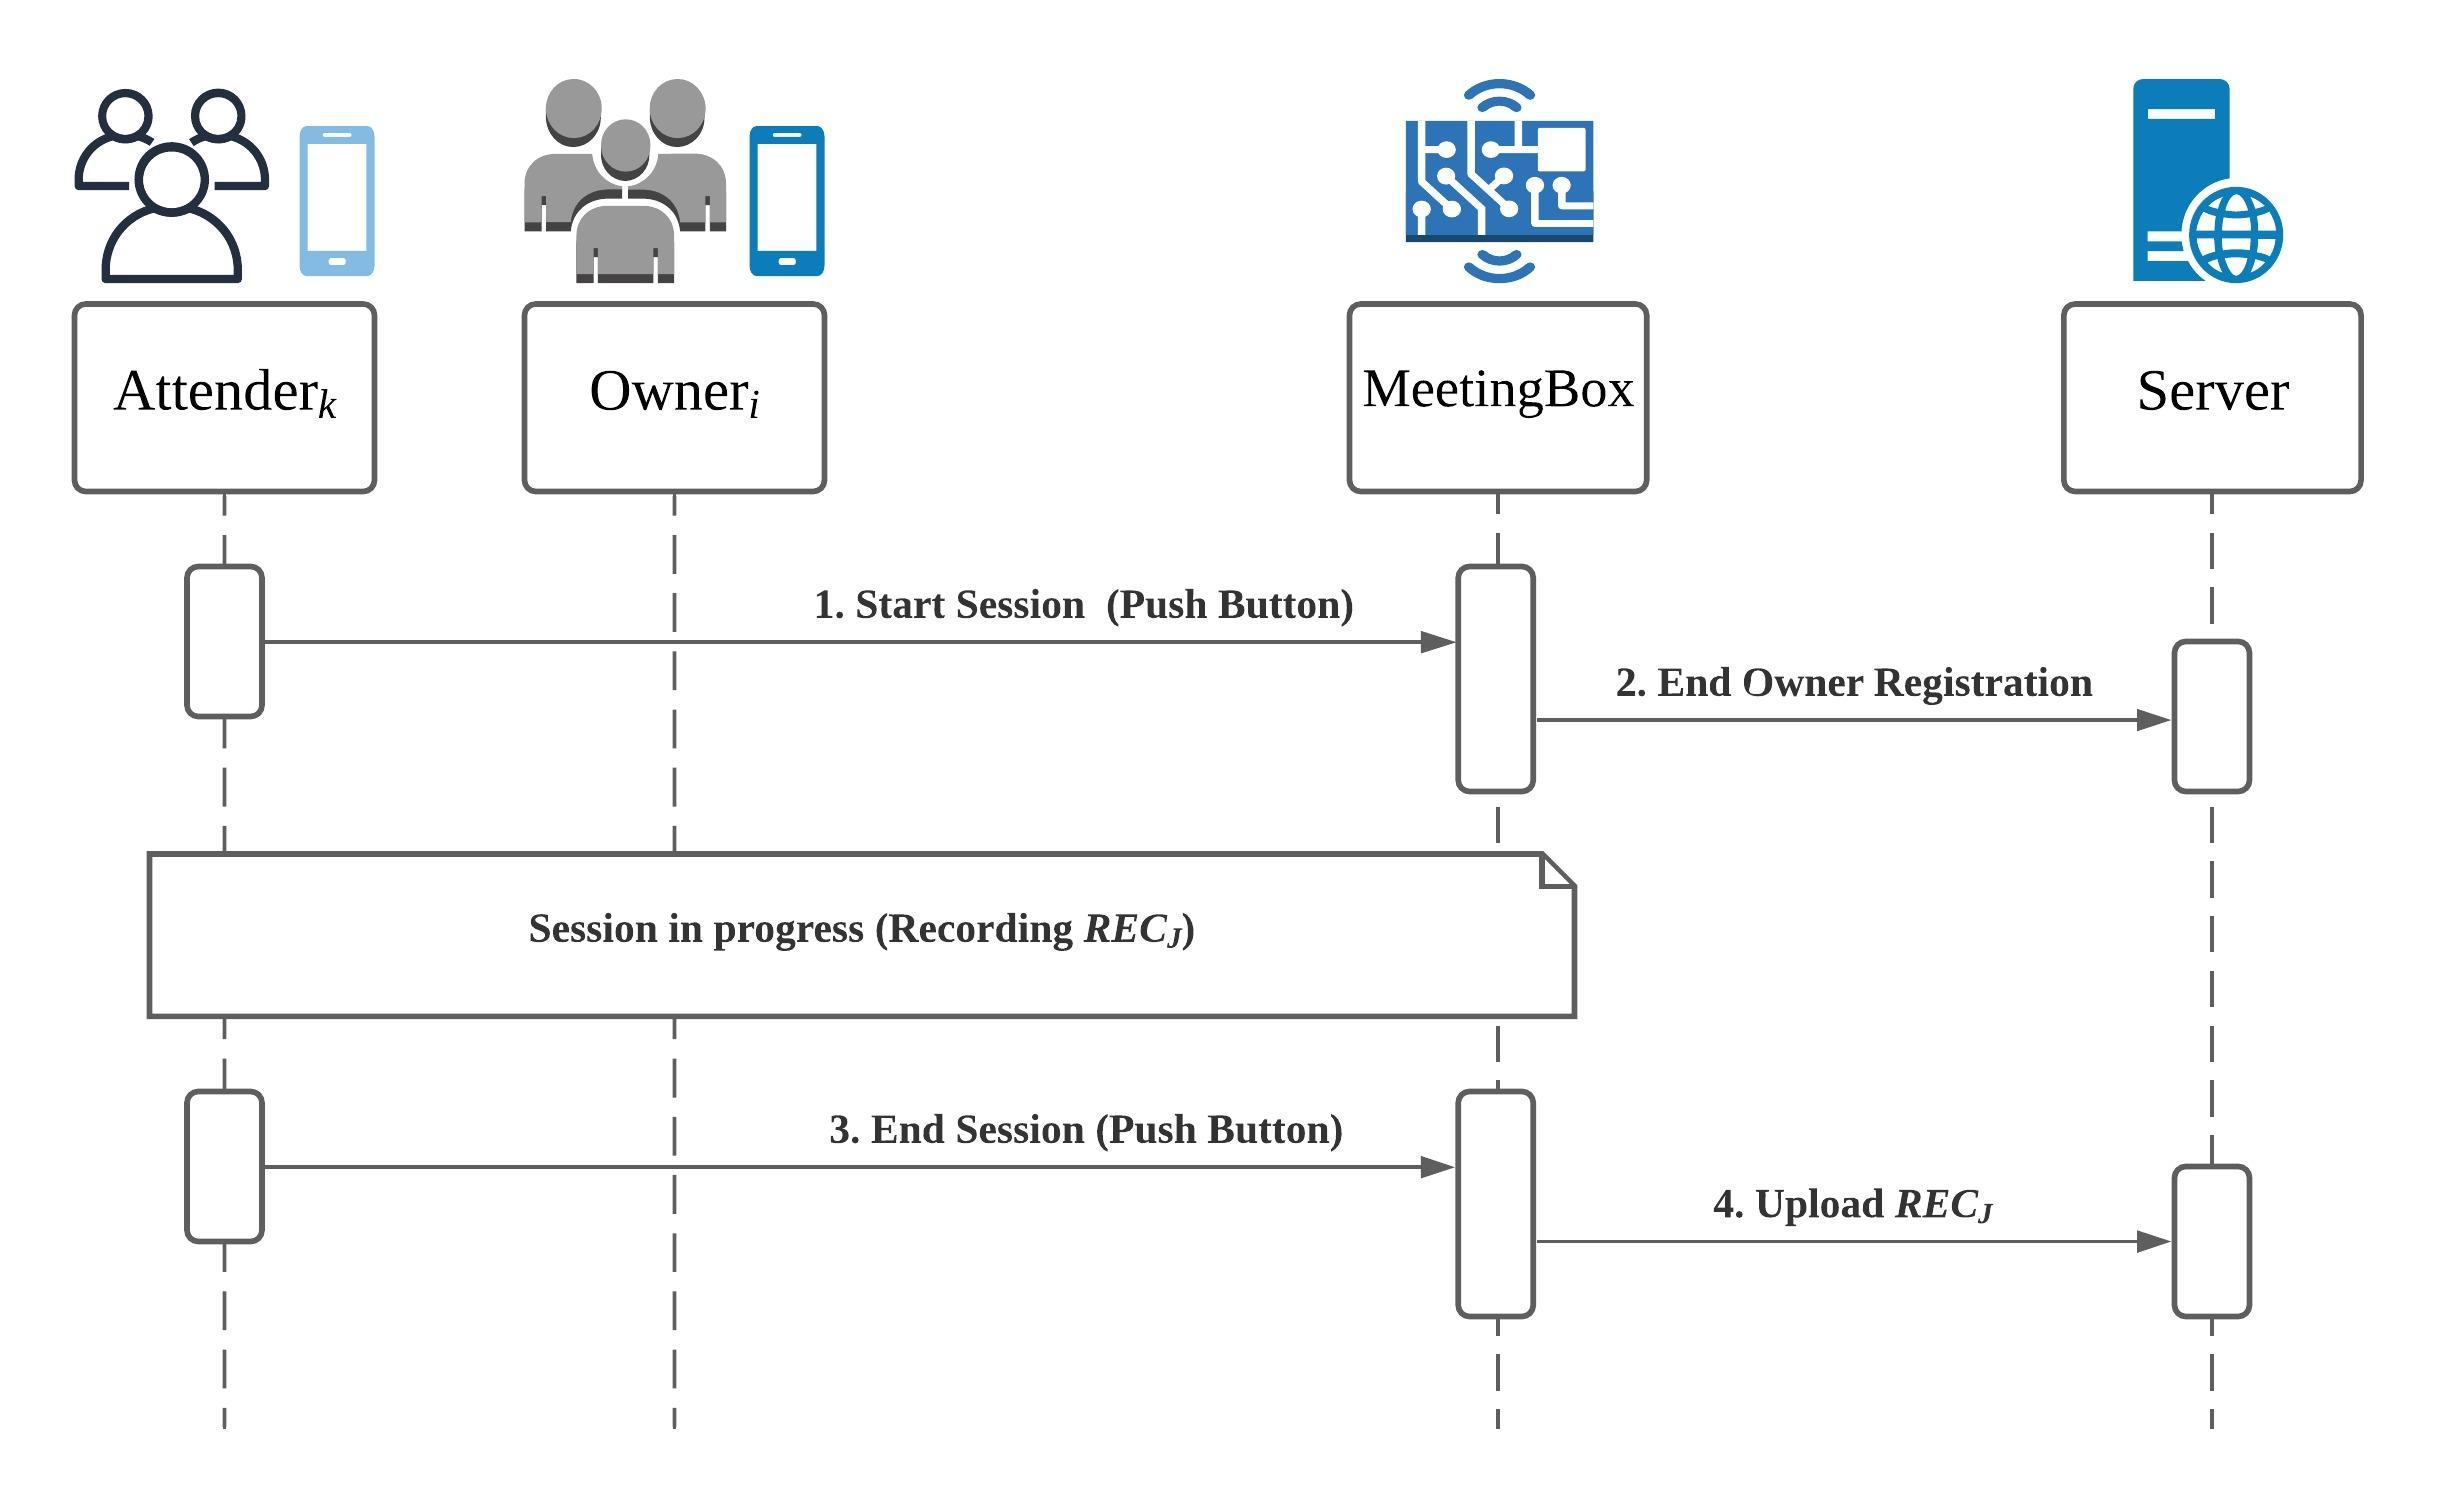
\includegraphics[width=0.9\textwidth]{multi-owner-sequence-diagram-sessioning}
    \caption{Multi Owner Running {\it Meeting Session}}
    \label{fig:m-o-sessioning}
\end{figure}

\begin{figure}[H]
    \centering
    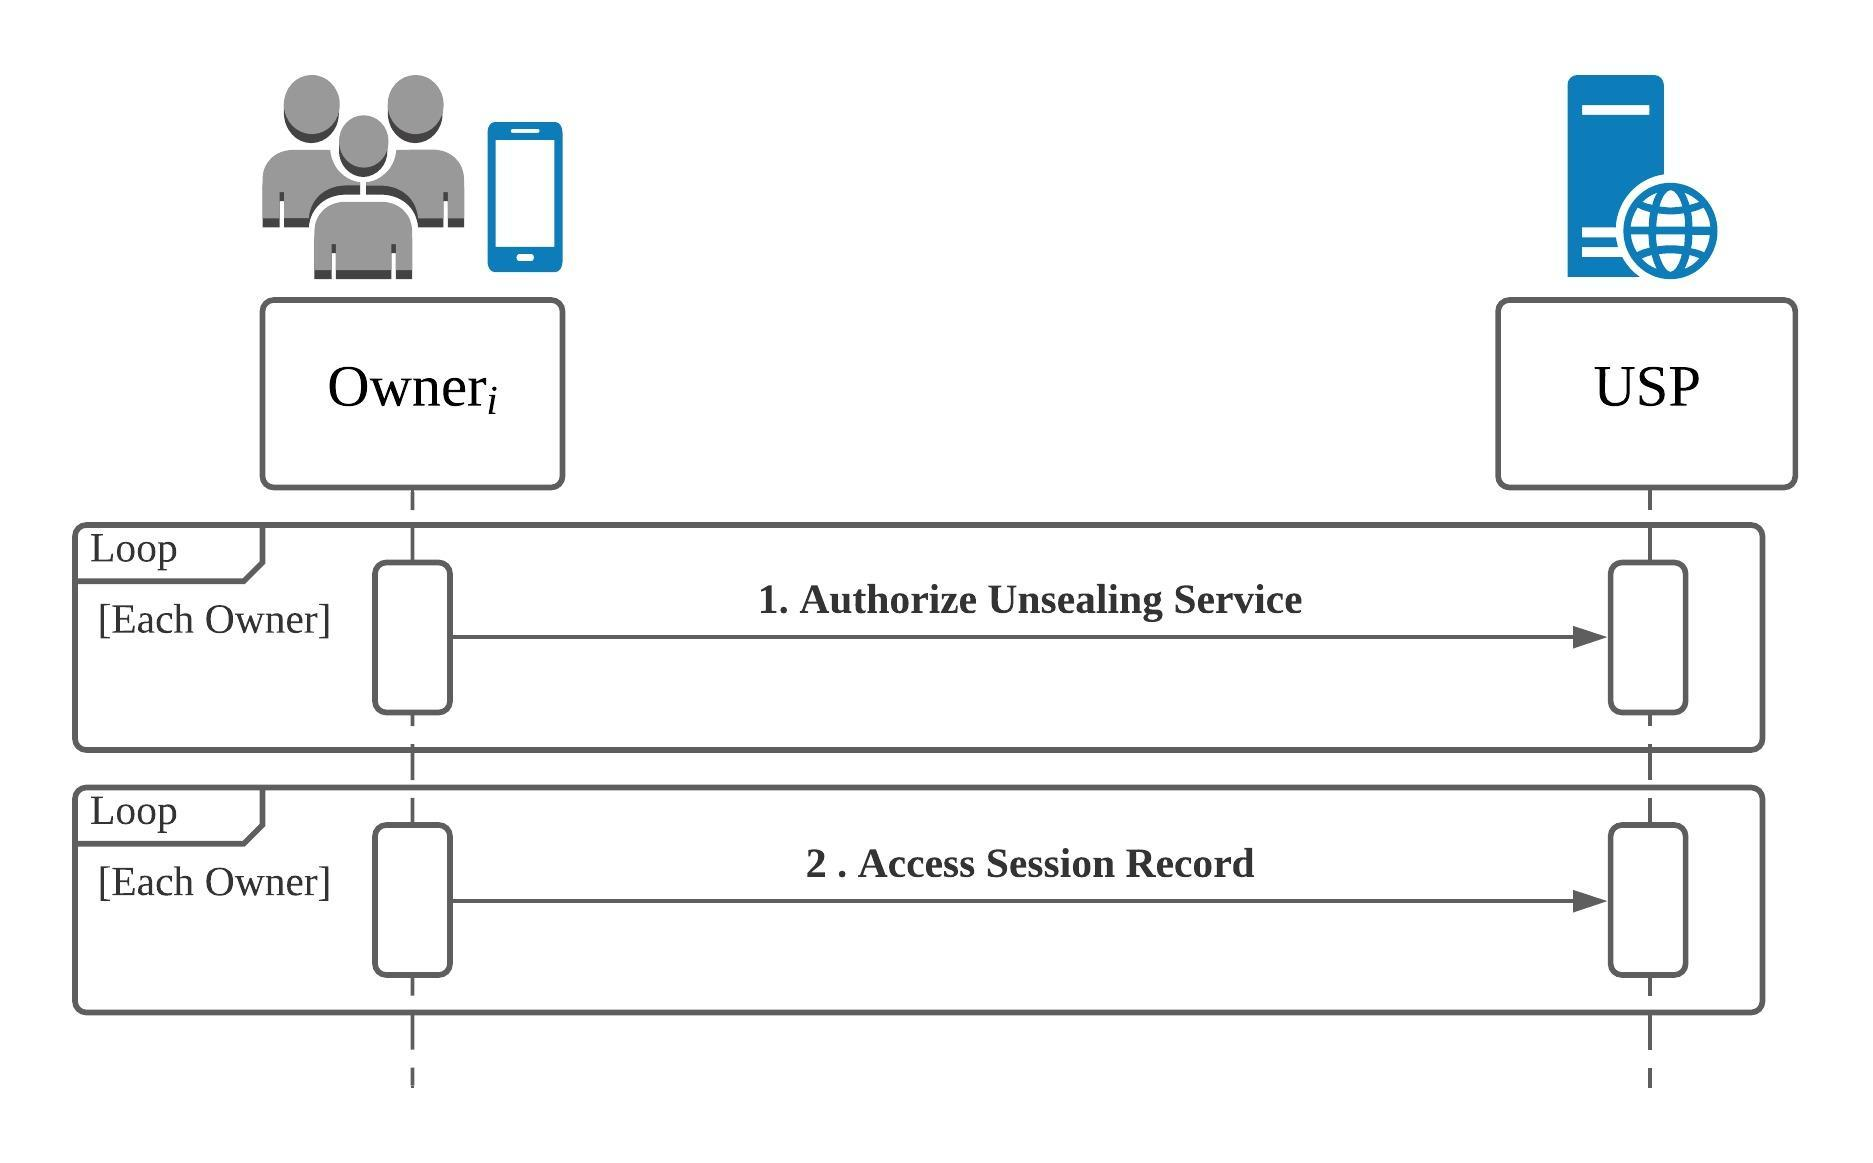
\includegraphics[width=0.7\textwidth]{multi-owner-sequence-diagram-unseal}
    \caption{Multi Owner {\it Unseal}}
    \label{fig:m-o-unseal}
\end{figure}


\section{系統機制之一:聲音記錄存取控制協定}
\label{sec:protocol}

    本節基於前章節 \ref{sec:system-flow} \nameref{sec:system-flow},延伸出一套聲音記錄存取控制協定。
其中包括創建會談、註冊會談主持者、進行會談、會談主持者授權解封伺服器、取得會談聲音記錄。


\subsection{創建會談機制之協定}

    在會談生命週期中初始化會談階段(圖\ref{fig:m-o-init}),當會談參與者透過與會談終端的物理控制介面執行創建會談,
會談終端獲得外部事件而觸發「\nameref{fig:protocol-init-create}」。
此協定為初始化會談中的 Step. 2\textasciitilde3,其運作細節如圖\ref{fig:protocol-init-create}與說明:

\begin{center}\scriptsize\setstretch{1}
\begin{tabularx}{0.95\textwidth} {
        |c
        >{\raggedright\arraybackslash}X
        >{\centering\arraybackslash}c
        >{\raggedright\arraybackslash}X
        c|
    }
    \hline

    \multicolumn{5}{|c|}{} \\
    & \multicolumn{1}{c}{\small{\DEFmeetingbox}} &
    & \multicolumn{1}{c}{\small{\DEFserver}} & \\
    %
    & \multicolumn{1}{c}{$\{$\DEFrecN$\}$} &
    & \multicolumn{1}{c}{} & \\
    %
    \cline{2-2} \cline{4-4}
    \multicolumn{5}{|c|}{} \\

    &
    $M_{1}$ $\leftarrow$ $\{\}$
    & & & \\

    & &
    $\xrightarrow{ \qquad M_{1} \qquad }$
    & & \\

    & & &
    \DEFsessionID $\leftarrow$ \DEFfuncIDgen{} \newline
    \DEFunsealKey $\leftarrow$ \DEFfuncKgen{} \newline
    \DEFowreg $\leftarrow$ $0$ \newline
    {\bf bind relations:} \newline
    \pcind \DEFunsealKey ~ $\in$ ~ \DEFsessionID \newline
    $M_{2}$ $\leftarrow$ $\{$\DEFsessionID, \DEFunsealKey$\}$
    & \\

    & &
    $\xleftarrow{ \qquad M_{2} \qquad }$
    & & \\

    &
    $k$ $\leftarrow$ \DEFunsealKey \newline
    $m_{3}$ $\leftarrow$ \DEFfuncEncEK{\DEFrecN} \newline
    $M_{3}$ $\leftarrow$ $\{$\DEFsessionID, $m_{3}$$\}$ \newline
    & & & \\

    & &
    $\xrightarrow{ \qquad M_{3} \qquad }$
    & & \\

    & & &
    \DEFrecP $\leftarrow$ $m_{3}$ \newline
    {\bf bind relations:} \newline
    \pcind \DEFrecP ~ $\in$ ~ \DEFsessionID \newline
    $M_{4}$ $\leftarrow$ $\{\}$
    & \\

    & &
    $\xleftarrow{ \qquad M_{4} \qquad }$
    & & \\

    &
    {\bf destroy~} \DEFunsealKey
    & & & \\

    \multicolumn{5}{|c|}{} \\
    \hline
\end{tabularx}
\captionof{figure}{創建會談機制之協定}\label{fig:protocol-init-create}
\setstretch{1.2}\normalsize\end{center}

\begin{pmsgs}
    \item $\{\}$ $,~$ \DEFmeetingbox $\rightarrow$ \DEFserver:

        當會談終端 \DEFmeetingbox 獲得外部事件,
    觸發會談終端向解封伺服器 \DEFserver 發送請求創建新的會談。

    \item $\{$\DEFsessionID, \DEFunsealKey$\}$ $,~$ \DEFserver $\rightarrow$ \DEFmeetingbox:

        解封伺服器 \DEFserver 收到訊息後,執行 \DEFfuncIDgen{} 與 \DEFfuncKgen{},
    分別產生此次會談的唯一識別碼 \DEFsessionID,與此次會談的解封金鑰 \DEFunsealKey。
    接著將 \DEFunsealKey 關聯綁定屬於 \DEFsessionID。
    接著建立一變數 \DEFowreg 定義為此會談的會談主持者於解封伺服器 \DEFserver 的註冊人數,初始值為 $0$。
    最後回傳 \DEFsessionID 與 \DEFunsealKey。

        其中 \DEFfuncKgen{} 為對稱式加密法的金鑰產生函數。
    \DEFfuncIDgen{} 為唯一識別碼產生函數,唯一識別碼的產生須滿足唯一性,隨機性,不可預測性。

    \item $\{$\DEFsessionID, \DEFrecP$\}$ $,~$ \DEFmeetingbox $\rightarrow$ \DEFserver:

        會談終端 \DEFmeetingbox 收到來自 \DEFserver 的回傳後,
    使用回傳的 \DEFunsealKey 透過對稱式加密函數 \DEFfuncEncEK{} 加密預先配置好的噪音 \DEFrecN,
    產生 \DEFrecP,接著向解封伺服器發出請求,訊息內容為 \DEFsessionID 與 \DEFrecP。

    \item $\{\}$ $,~$ \DEFserver $\rightarrow$ \DEFmeetingbox:

        解封伺服器 \DEFserver 收到訊息後,將 \DEFrecP 關聯綁定屬於 \DEFsessionID。
    隨後回覆會談終端 \DEFmeetingbox 上傳成功。
    會談終端 \DEFmeetingbox 收到來自解封伺服器 \DEFserver 的上傳成功回覆後,
    銷毀於會談終端上的 \DEFrecN 與 \DEFunsealKey。
\end{pmsgs}


\subsection{註冊會談主持者機制之協定}

    於會談生命週期同一階段初始化會談中,當談終端 \DEFmeetingbox 獲得產自解封伺服器的 \DEFsessionID 後,
會談終端上的人機互動介面提示,可以進行「\nameref{fig:protocol-init-reg}」。

    此協定需要所有的會談主持者 \DEFownerAll 執行,各會談主持者 \DEFowner 可以同時獨立執行,
每個會談主持者 \DEFowner 的執行結果不受其他會談主持者影響。
此協定為初始化會談中的 Step. 4\textasciitilde5,其運作細節如圖\ref{fig:protocol-init-reg}與說明:

\begin{center}\scriptsize\setstretch{1}
\begin{tabularx}{0.95\textwidth} {
        |c
        >{\raggedright\arraybackslash}X
        >{\centering\arraybackslash}c
        >{\raggedright\arraybackslash}X
        >{\centering\arraybackslash}c
        >{\raggedright\arraybackslash}X
        c|
    }
    \hline

    \multicolumn{7}{|c|}{} \\
    & \multicolumn{1}{c}{\small{\DEFowner}} &
    & \multicolumn{1}{c}{\small{\DEFmeetingbox}} &
    & \multicolumn{1}{c}{\small{\DEFserver}} & \\
    %
    & \multicolumn{1}{c}{} &
    & \multicolumn{1}{c}{$\{$\DEFsessionID$\}$} &
    & \multicolumn{1}{c}{$\{$\DEFsessionID, \DEFowreg$\}$} & \\
    %
    \cline{2-2} \cline{4-4} \cline{6-6}
    \multicolumn{7}{|c|}{} \\

    & {\bf for each~} \DEFowner $\in$ \DEFownerAll \newline
    \pcind {\bf where~} $i=1~...\mid$\DEFownerAll$\mid$ {\bf:}
    & & & & & \\

    \cdashline{2-6}

    \rule{0pt}{10pt} & \multicolumn{1}{:l}{
    \pcind\pcind $M_{1}^{i}$ $\leftarrow$ $\{\}$
    } & & & & \multicolumn{1}{l:}{} & \\

    & \multicolumn{1}{:l}{} &
    $\xrightarrow{ \enskip M_{1}^{i} \enskip }$
    & & & \multicolumn{1}{l:}{} & \\

    & \multicolumn{1}{:l}{} & &
    $M_{2}^{i}$ $\leftarrow$ $\{$\DEFsessionID$\}$
    & $\quad\quad\quad\quad$ & \multicolumn{1}{l:}{} & \\

    & \multicolumn{1}{:l}{} &
    $\xleftarrow{ \enskip M_{2}^{i} \enskip }$
    & & & \multicolumn{1}{l:}{} & \\

    & \multicolumn{1}{:l}{
    \pcind\pcind $M_{3}^{i}$ $\leftarrow$ $\{$\DEFsessionID$\}$
    } & & & & \multicolumn{1}{l:}{} & \\

    & \multicolumn{1}{:l}{} & \multicolumn{3}{c}{
    $\xrightarrow{\qquad\qquad\qquad\qquad\qquad M_{3}^{i} \qquad\qquad\qquad\qquad\qquad}$
    }& \multicolumn{1}{l:}{} & \\

    & \multicolumn{1}{:l}{} & & & & \multicolumn{1}{l:}{\shortstack[l]{
    $($\DEFpublicKey, \DEFprivateKey$)$ $\leftarrow$ \DEFfuncPKgen{} \\
    \DEFownerID $\leftarrow$ \DEFfuncIDgen{}{} \\
    {\bf bind relations:} \\
    \pcind \DEFownerID $\in$ \DEFsessionID \\
    \pcind \DEFpublicKey $\in$ \DEFownerID \\
    \DEFowreg $\leftarrow$ \DEFowreg $+1$ \\
    $M_{4}^{i}$ $\leftarrow$ $\{$\DEFownerID, \DEFprivateKey$\}$
    }} & \\

    & \multicolumn{1}{:l}{} & \multicolumn{3}{c}{
    $\xleftarrow{\qquad\qquad\qquad\qquad\qquad M_{4}^{i} \qquad\qquad\qquad\qquad\qquad}$
    }& \multicolumn{1}{l:}{} & \\

    & \multicolumn{1}{:l}{
    \pcind\pcind {\bf store~} $\{$\DEFownerID, \DEFprivateKey$\}$
    } & & & & \multicolumn{1}{l:}{
    {\bf destroy~} \DEFprivateKey
    } & \\

    & \multicolumn{1}{:l}{} & & & & \multicolumn{1}{l:}{} & \\
    \cdashline{2-6}

    \multicolumn{7}{|c|}{} \\
    \hline
\end{tabularx}
\captionof{figure}{註冊會談主持者機制之協定}\label{fig:protocol-init-reg}
\setstretch{1.2}\normalsize\end{center}

\begin{pmsgsi}
    \item $\{\}$ $,~$ \DEFowner $\rightarrow$ \DEFmeetingbox:

        當會談主持者 \DEFowner 觀察到於會談終端 \DEFmeetingbox 上的人機互動介面提示,
    向發會談終端送此請求,以獲得會談的元資料。

    \item $\{$\DEFsessionID$\}$ $,~$ \DEFmeetingbox $\rightarrow$ \DEFowner:

        會談終端 \DEFmeetingbox 收到請求後,回覆 \DEFsessionID,傳遞此次會談的元資料給會談主持者 \DEFowner。

    \item $\{$\DEFsessionID$\}$ $,~$ \DEFowner $\rightarrow$ \DEFserver:

        會談主持者 \DEFowner 獲得此次會談的元資料 \DEFsessionID 後,便可向解封伺服器 \DEFserver 傳送註冊請求,
    訊息內容為 \DEFsessionID。

        解封伺服器 \DEFserver 收到註冊請求後,執行 \DEFfuncPKgen{} 與 \DEFfuncIDgen{},
    分別產生一組屬於會談主持者 \DEFowner 的公開私密金鑰對 $($\DEFpublicKey$,~$ \DEFprivateKey$)$,
    與此會談主持者 \DEFowner 的唯一識別碼 \DEFownerID。
    會談主持者的唯一識別碼 \DEFownerID,其產生須滿足唯一性,隨機性,不可預測性。
    \DEFfuncPKgen{} 為非對稱加密演算法的公開私密金鑰對產生函數。

        接著將此次會談的會談主持者註冊人數 \DEFowreg 遞增 $1$,
    並將 \DEFownerID 關聯綁定屬於 \DEFsessionID,\DEFpublicKey 關聯綁定屬於 \DEFownerID 並儲存。
    隨後回傳 \DEFownerID 與其私鑰 \DEFprivateKey,並銷毀 \DEFprivateKey。

    \item $\{$\DEFownerID, \DEFprivateKey$\}$ $,~$ \DEFserver $\rightarrow$ \DEFowner:

        會談主持者收到解封伺服器 \DEFserver 的回傳即註冊成功。
    會談主持者為會談參與者中的特權角色,其特權來源為會傳訊息內的 \DEFprivateKey,
    因此會談主持者須妥善保管 \DEFprivateKey,維持其機密性。
    待所有的會談主持者 \DEFownerAll 執行成功此機制後,即完成會談初始化。
\end{pmsgsi}


\subsection{進行會談機制之協定}

    在會談生命週期中進行會談階段(圖\ref{fig:m-o-sessioning}),
會談參與者透過與會談終端的物理控制介面(Step. 1、3),
使會談終端獲得外部事件而觸發「\nameref{fig:protocol-init-create}」。

    在此機制中,會談已完成會談生命週期第一階段初始化會談。此時會談終端應已獲得此次會談唯一識別碼 \DEFsessionID。
解封伺服器 \DEFserver 中也應存在資料包含會談主持者註冊人數 \DEFowreg、
屬於此次會談唯一識別碼的所有會談主持者唯一識別碼 \DEFownerID 與其 \DEFpublicKey。

    此機制完成後系統將產生被干擾的會談聲音記錄 \DEFrecJ 與受加密保護的授權金鑰 \DEFakEnc。
其運作細節如圖\ref{fig:protocol-sessioning}與說明:

\begin{center}\scriptsize\setstretch{1}
\begin{tabularx}{0.95\textwidth} {
        |c
        >{\raggedright\arraybackslash}X
        >{\centering\arraybackslash}c
        >{\raggedright\arraybackslash}X
        c|
    }
    \hline

    \multicolumn{5}{|c|}{} \\
    & \multicolumn{1}{c}{\small{\DEFmeetingbox}} &
    & \multicolumn{1}{c}{\small{\DEFserver}} & \\
    %
    & \multicolumn{1}{c}{$\{$\DEFsessionID, \DEFrecJ$\}$} &
    & \multicolumn{1}{c}{$\{$
        \DEFsessionID,
        \DEFowreg,
        $\{[($ \DEFownerID, \DEFpublicKey $)] \mid i=1~...$\DEFowreg $\}\}$}
    & \\
    %
    \cline{2-2} \cline{4-4}
    \multicolumn{5}{|c|}{} \\

    &
    $M_{1}$ $\leftarrow$ $\{$\DEFsessionID$\}$
    & & & \\

    & &
    $\xrightarrow{ \enskip M_{1} \enskip }$
    & & \\

    & & &
    {\bf if~} \DEFowreg $=1${\bf:} \newline
    \pcind $pk$ $\leftarrow$ \DEFpublicKey \newline
    \pcind \DEFakEnc $\leftarrow$ \DEFfuncEncPK{\DEFunsealKey} \newline
    \pcind {\bf bind relations:} \newline
    \pcind\pcind \DEFakEnc $\in$ \DEFownerID \newline

    {\bf if~} \DEFowreg $>1${\bf:} \newline
    \pcind $c$ $\leftarrow$ \DEFowreg \newline
    \pcind $t$ $\leftarrow$ \DEFowreg \newline
    \pcind $[s_{i}]$ $\leftarrow$ \DEFfuncSSS{\DEFunsealKey} \newline
    \pcind {\bf for each~} $s_{i} \in [s_{i}]$~ {\bf where~} $i=1~...$\DEFowreg {\bf:} \newline
    \pcind\pcind $pk$ $\leftarrow$ \DEFpublicKey \newline
    \pcind\pcind \DEFakEnc $\leftarrow$ \DEFfuncEncPK{$s_{i}$} \newline
    \pcind\pcind {\bf destroy~} $s_{i}$ \newline
    \pcind\pcind {\bf bind relations:} \newline
    \pcind\pcind\pcind \DEFakEnc $\in$ \DEFownerID \newline

    {\bf destroy~} \DEFunsealKey \newline
    $M_{2}$ $\leftarrow$ $\{\}$
    & \\

    & &
    $\xleftarrow{ \enskip M_{2} \enskip }$
    & & \\

    \multicolumn{5}{|c|}{} \\
    \cline{2-2}
    & \multicolumn{1}{|c|}{} & & & \\
    & \multicolumn{1}{|c|}{Session in progress (Recording \DEFrecJ)} & & & \\
    & \multicolumn{1}{|c|}{} & & & \\
    \cline{2-2}
    \multicolumn{5}{|c|}{} \\

    &
    $M_{3}$ $\leftarrow$ $\{$\DEFsessionID, \DEFrecJ$\}$
    & & & \\

    & &
    $\xrightarrow{ \enskip M_{3} \enskip }$
    & & \\

    & & &
    {\bf bind relations:} \newline
    \pcind \DEFrecJ ~ $\in$ ~ \DEFsessionID \newline
    $M_{4}$ $\leftarrow$ $\{\}$
    & \\

    & &
    $\xleftarrow{ \enskip M_{4} \enskip }$
    & & \\

    \multicolumn{5}{|c|}{} \\
    \hline
\end{tabularx}
\captionof{figure}{進行會談機制之協定}\label{fig:protocol-sessioning}
\setstretch{1.2}\normalsize\end{center}

\begin{pmsgs}
    \item $\{$\DEFsessionID$\}$ $,~$ \DEFmeetingbox $\rightarrow$ \DEFserver:

        會談參與者透過與會談終端的物理控制介面,
    使會談終端 \DEFmeetingbox 獲得外部事件而觸發向解封伺服器 \DEFserver 發出此請求,
    通知 \DEFserver,會談主持者註冊已完成。請求內容為此次會談唯一識別碼 \DEFsessionID。

    \item $\{\}$ $,~$ \DEFserver $\rightarrow$ \DEFmeetingbox:

        解封伺服器收到會談終端的請求後,即終止此會談不再有新的會談擁有者註冊。
    因此會談唯一識別 \DEFsessionID 限制不再新增關聯綁定。
    接著判斷會談主持者註冊人數 \DEFowner 是否為一或多人。

        若為一人,則為單一會談主持者情境。此時將屬於此會議的解封金鑰 \DEFunsealKey,
    透過唯一會談主持者 \DEFowner 的非對稱是公開金鑰 \DEFpublicKey,
    使用非對稱式金鑰演算法加密函數 \DEFfuncEncPK{} 加密。因僅有單一會談主持者,
    加密後的解封金鑰 \DEFunsealKey,則視為唯一會談主持者 \DEFowner 的受加密保護的授權金鑰 \DEFakEnc。

        若為多人,則為多會談主持者情境。此時將屬於此會議的解封金鑰 \DEFunsealKey,
    透過金鑰分割函數 \DEFfuncSSS{},根據會談主持者註冊人數 \DEFowreg,
    分割成 \DEFowreg 份分割秘密 \DEFsharesAll。
    再將每個分割秘密 \DEFshares,透過每個會談主持者 \DEFowner 的公開金鑰 \DEFpublicKey,
    使用非對稱式金鑰演算法加密函數 \DEFfuncEncPK{} 加密,並銷毀該分割秘密。
    受加密保護的分割秘密,即定義為該會談主持者 \DEFowner 的受加密保護的授權金鑰 \DEFakEnc。

        當所有會談主持者 \DEFowner 的受加密保護的授權金鑰 \DEFakEnc 產生完畢。
    隨即銷毀該會談的解封金鑰 \DEFunsealKey,並回覆註冊終止成功。
    會談終端 \DEFmeetingbox 收到解封伺服器的回覆後,終止註冊完成。
    此時開起會談終端上的超音波麥克風干擾器與麥克風,開始錄製受干擾的會談聲音 \DEFrecJ

    \item $\{$\DEFsessionID, \DEFrecJ$\}$ $,~$ \DEFmeetingbox $\rightarrow$ \DEFserver:

        當會談參與者再次透過與會談終端的物理控制介面,
    使會談終端 \DEFmeetingbox 獲得外部事件,此時觸發會談錄音終止,受干擾的會談聲音紀錄 \DEFrecJ 產生完成。
    會談終端 \DEFmeetingbox 向解封伺服器 \DEFserver 發出請求上傳,
    內容為此次會談唯一識別碼 \DEFsessionID 與受干擾的會談聲音紀錄 \DEFrecJ。

    \item $\{\}$ $,~$ \DEFserver $\rightarrow$ \DEFmeetingbox:

        解封伺服器收到會談終端的請求後,
    將受干擾的會談聲音紀錄 \DEFrecJ 關聯綁定屬於 \DEFsessionID 且儲存,隨後回覆上傳成功。
    此時會談參與者即可離開會談場域,會談終端開始為未來新的會談生命週期重新配置。
\end{pmsgs}


\subsection{會談主持者授權解封伺服器機制之協定}

\begin{center}\scriptsize\setstretch{1}
\begin{tabularx}{0.95\textwidth} {
        |c
        >{\raggedright\arraybackslash}X
        >{\centering\arraybackslash}c
        >{\raggedright\arraybackslash}X
        c|
    }
    \hline

    \multicolumn{5}{|c|}{} \\
    & \multicolumn{1}{c}{\small{\DEFowner}} &
    & \multicolumn{1}{c}{\small{\DEFserver}} & \\
    %
    & \multicolumn{1}{c}{$\{$ \DEFsessionID,
        $\{[($ \DEFownerID, \DEFprivateKey $)] \mid i=1~...\mid$\DEFownerAll$\mid$ $\}\}$}
    & & \multicolumn{1}{c}{\shortstack[c]{$\{$
        \DEFsessionID,
        $\{[($ \DEFownerID, \DEFpublicKey, \DEFakEnc $)] \mid i=1~...$\DEFowreg $\}\}$}}
    & \\
    %
    \cline{2-2} \cline{4-4}
    \multicolumn{5}{|c|}{} \\

    & {\bf for each~} \DEFowner $\in$ \DEFownerAll \newline
    \pcind {\bf where~} $i=1~...\mid$\DEFownerAll$\mid$ {\bf:}
    & & & \\

    \cdashline{2-4}

    \rule{0pt}{10pt} & \multicolumn{1}{:l}{
    \pcind\pcind $M_{1}^{i}$ $\leftarrow$ $\{$\DEFsessionID, \DEFownerID$\}$
    } & & \multicolumn{1}{l:}{} & \\

    & \multicolumn{1}{:l}{} &
    $\xrightarrow{ \enskip M_{1}^{i} \enskip }$
    & \multicolumn{1}{l:}{} & \\

    & \multicolumn{1}{:l}{} & & \multicolumn{1}{l:}{
    $M_{2}^{i}$ $\leftarrow$ $\{$\DEFownerID, \DEFakEnc$\}$
    } & \\

    & \multicolumn{1}{:l}{} &
    $\xleftarrow{ \enskip M_{2}^{i} \enskip }$
    & \multicolumn{1}{l:}{} & \\

    & \multicolumn{1}{:l}{\shortstack[l]{
    \pcind\pcind $sk$ $\leftarrow$ \DEFprivateKey \\
    \pcind\pcind $m_{3}$ $\leftarrow$ \DEFfuncDecSK{\DEFakEnc} \\
    \pcind\pcind $m_{3}.sig$ $\leftarrow$ \DEFfuncSignSK{$m_{3}$} \\
    \pcind\pcind $M_{3}^{i}$ $\leftarrow$ $\{m_{3}, ~m_{3}.sig\}$
    }} & & \multicolumn{1}{l:}{} & \\

    & \multicolumn{1}{:l}{} &
    $\xrightarrow{ \enskip M_{3}^{i} \enskip }$
    & \multicolumn{1}{l:}{} & \\

    & \multicolumn{1}{:l}{} & & \multicolumn{1}{l:}{\shortstack[l]{
    $pk$ $\leftarrow$ \DEFpublicKey \\
    $valid$ $\leftarrow$ \DEFfuncVerfPK{$m_{3},~m_{3}.sig$} \\
    {\bf if} !$valid$ {\bf :} \\
    \pcind {\bf terminate session} \\
    {\bf else} {\bf :} \\
    \pcind \DEFagentKey $\leftarrow$ $m_{3}$ \\
    \pcind {\bf bind relations:} \\
    \pcind\pcind \DEFagentKey $\in$ \DEFownerID \\
    $M_{4}^{i}$ $\leftarrow$ $\{\}$
    }} & \\

    & \multicolumn{1}{:l}{} &
    $\xleftarrow{ \enskip M_{4}^{i} \enskip }$
    & \multicolumn{1}{l:}{} & \\

    & \multicolumn{1}{:l}{} & & \multicolumn{1}{l:}{} & \\
    \cdashline{2-4}

    \multicolumn{5}{|c|}{} \\
    \hline
\end{tabularx}
\captionof{figure}{會談主持者授權解封伺服器機制之協定}\label{fig:protocol-unseal-auth}
\setstretch{1.2}\normalsize\end{center}

\begin{pmsgsi}
    \item \DEFowner $\rightarrow$ \DEFserver:



    \item \DEFserver $\rightarrow$ \DEFowner:

    \item \DEFowner $\rightarrow$ \DEFserver:

    \item \DEFserver $\rightarrow$ \DEFowner:

\end{pmsgsi}


\subsection{取得會談聲音記錄機制之協定}

\begin{center}\scriptsize\setstretch{1}
\begin{tabularx}{0.95\textwidth} {
        |c
        >{\raggedright\arraybackslash}X
        >{\centering\arraybackslash}c
        >{\raggedright\arraybackslash}X
        c|
    }
    \hline

    \multicolumn{5}{|c|}{} \\
    & \multicolumn{1}{c}{\small{\DEFowner}} &
    & \multicolumn{1}{c}{\small{\DEFserver}} & \\
    %
    & \multicolumn{1}{c}{$\{$\DEFsessionID$\}$}
    & & \multicolumn{1}{c}{\shortstack[c]{$\{$
        \DEFsessionID, \DEFowreg, \DEFrecP, \DEFrecJ, \\
        $\{[($ \DEFownerID, \DEFagentKey $)] \mid i=1~...$\DEFowreg $\}\}$}}
    & \\
    %
    \cline{2-2} \cline{4-4}
    \multicolumn{5}{|c|}{} \\
    
    &
    $M_{1}$ $\leftarrow$ $\{$\DEFsessionID$\}$
    & & & \\

    & &
    $\xrightarrow{ \qquad M_{1} \qquad }$
    & & \\

    & & &
    {\bf if~} \DEFowreg $=1${\bf:} \newline
    \pcind \DEFunsealKey $\leftarrow$ \DEFagentKey \newline

    {\bf if~} \DEFowreg $>1${\bf:} \newline
    \pcind $[s_{i}]$ $\leftarrow$ $\{[$ \DEFagentKey $] \mid i=1~...$\DEFowreg $\}$ \newline
    \pcind \DEFunsealKey $\leftarrow$ \DEFfuncSSC{$[s_{i}]$} \newline

    $k$ $\leftarrow$ \DEFunsealKey \newline
    \DEFrecN $\leftarrow$ \DEFfuncDecEK{\DEFrecP} \newline
    \DEFshift $\leftarrow$ \DEFfuncEstm{\DEFrecJ,~\DEFrecN} \newline
    \DEFrecREV $\leftarrow$ \DEFfuncAnc{\DEFrecJ,~\DEFrecN} \newline
    $M_{2}$ $\leftarrow$ $\{$\DEFsessionID,\DEFrecREV$\}$
    & \\

    & &
    $\xleftarrow{ \qquad M_{2} \qquad }$
    & & \\

    &
    {\bf output~} \DEFrecREV
    & & & \\

    \multicolumn{5}{|c|}{} \\
    \hline
\end{tabularx}
\captionof{figure}{取得會談聲音記錄機制之協定}\label{fig:protocol-unseal-access}
\setstretch{1.2}\normalsize\end{center}

\begin{pmsgs}
    \item \DEFowner $\rightarrow$ \DEFserver:

    \item \DEFserver $\rightarrow$ \DEFowner:

\end{pmsgs}


\section{系統機制之二:自適應噪音消除}
\label{sec:anc}

    本節將說明於生命週期解封會談錄音中,如何應用自適應噪音消除,以還原出有效的會談錄音。

\begin{figure}[H]
    \centering
    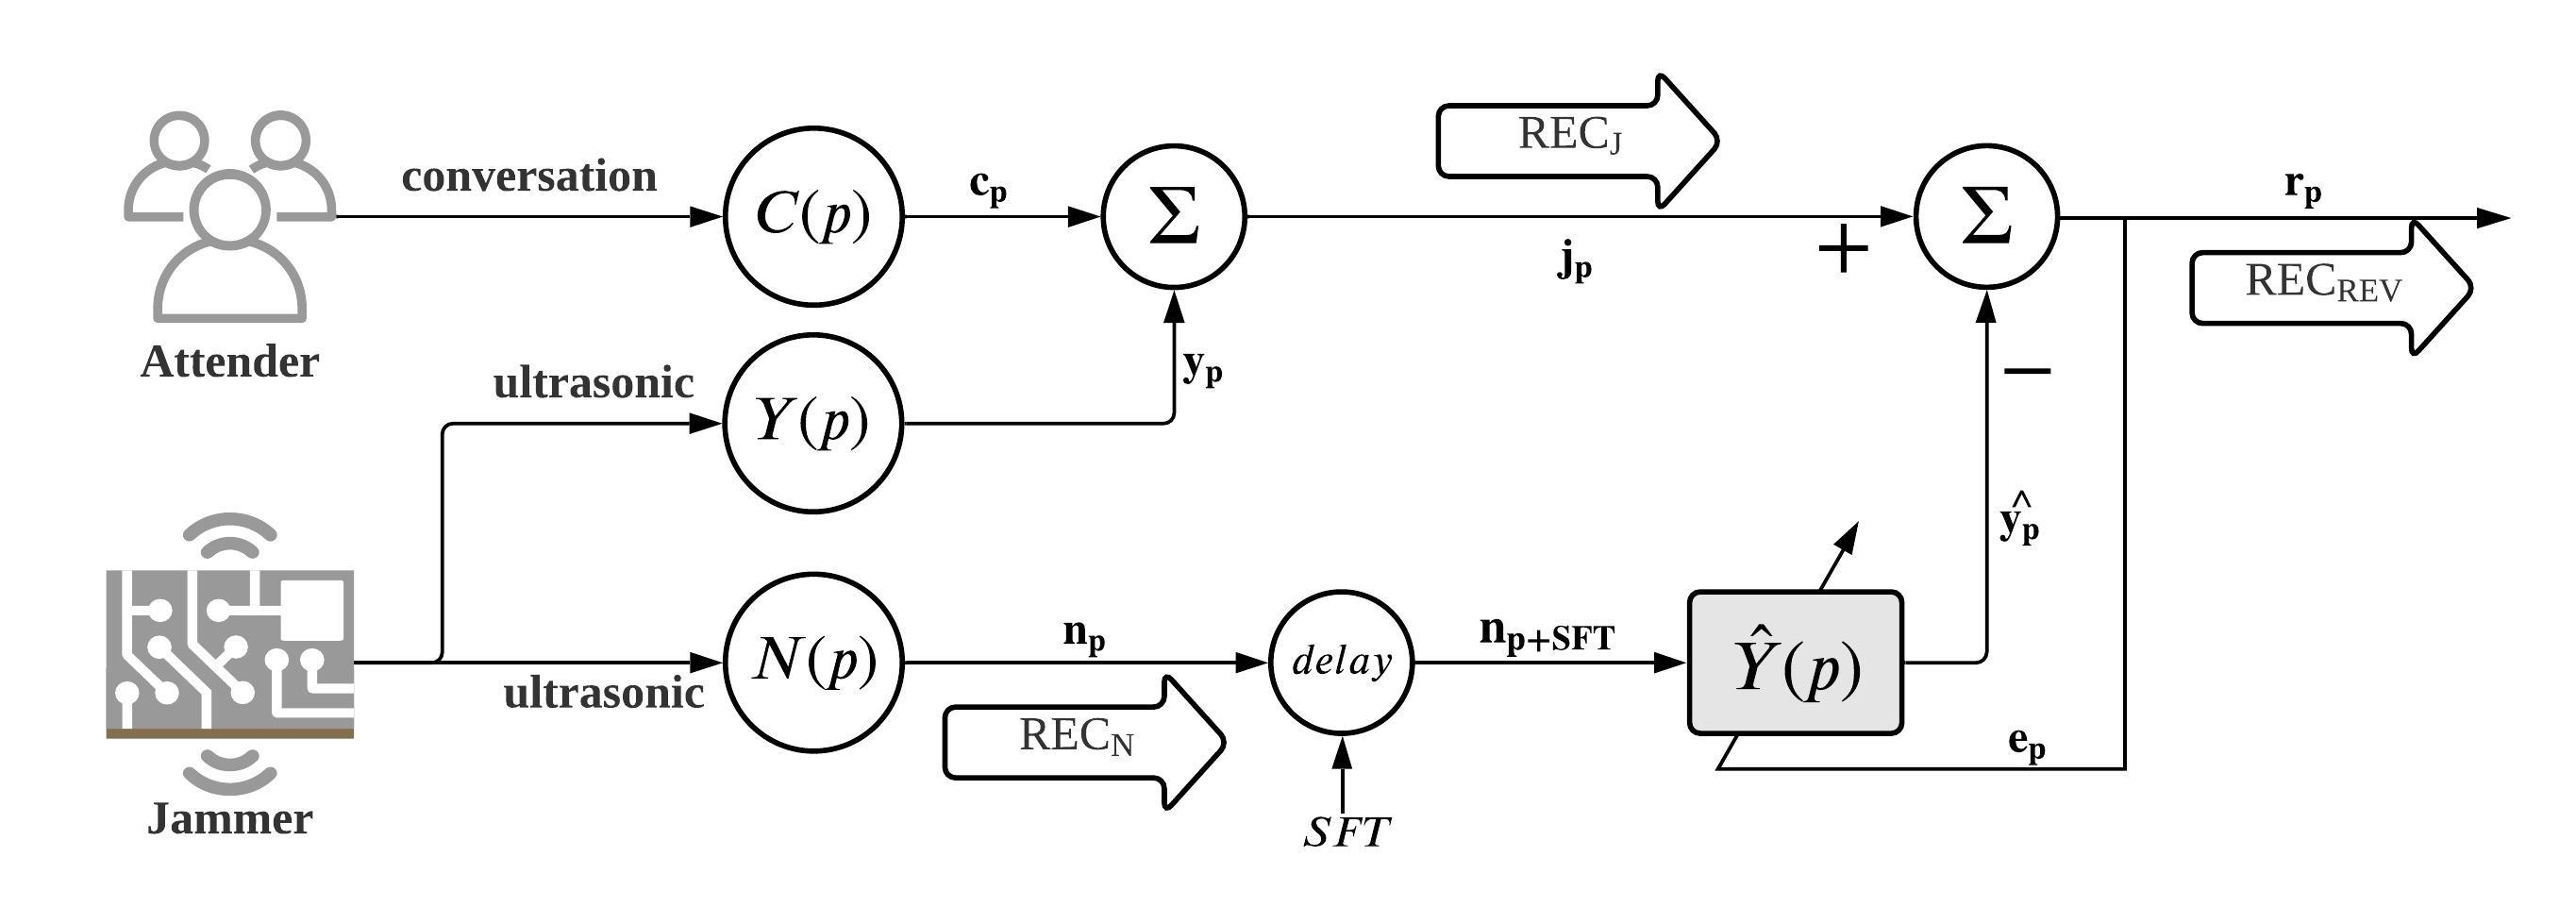
\includegraphics[width=1.0\textwidth]{anc}
    \caption{自適應噪音消除}
    \label{fig:anc}
\end{figure}


\section{系統機制之三:聲音樣本的離散時間誤差推估}
\label{sec:estimate}

    本節將說明如何推估聲音樣本的離散時間誤差值,用於自適應噪音消除時對齊聲音樣本。

\begin{figure}[H]
    \centering
    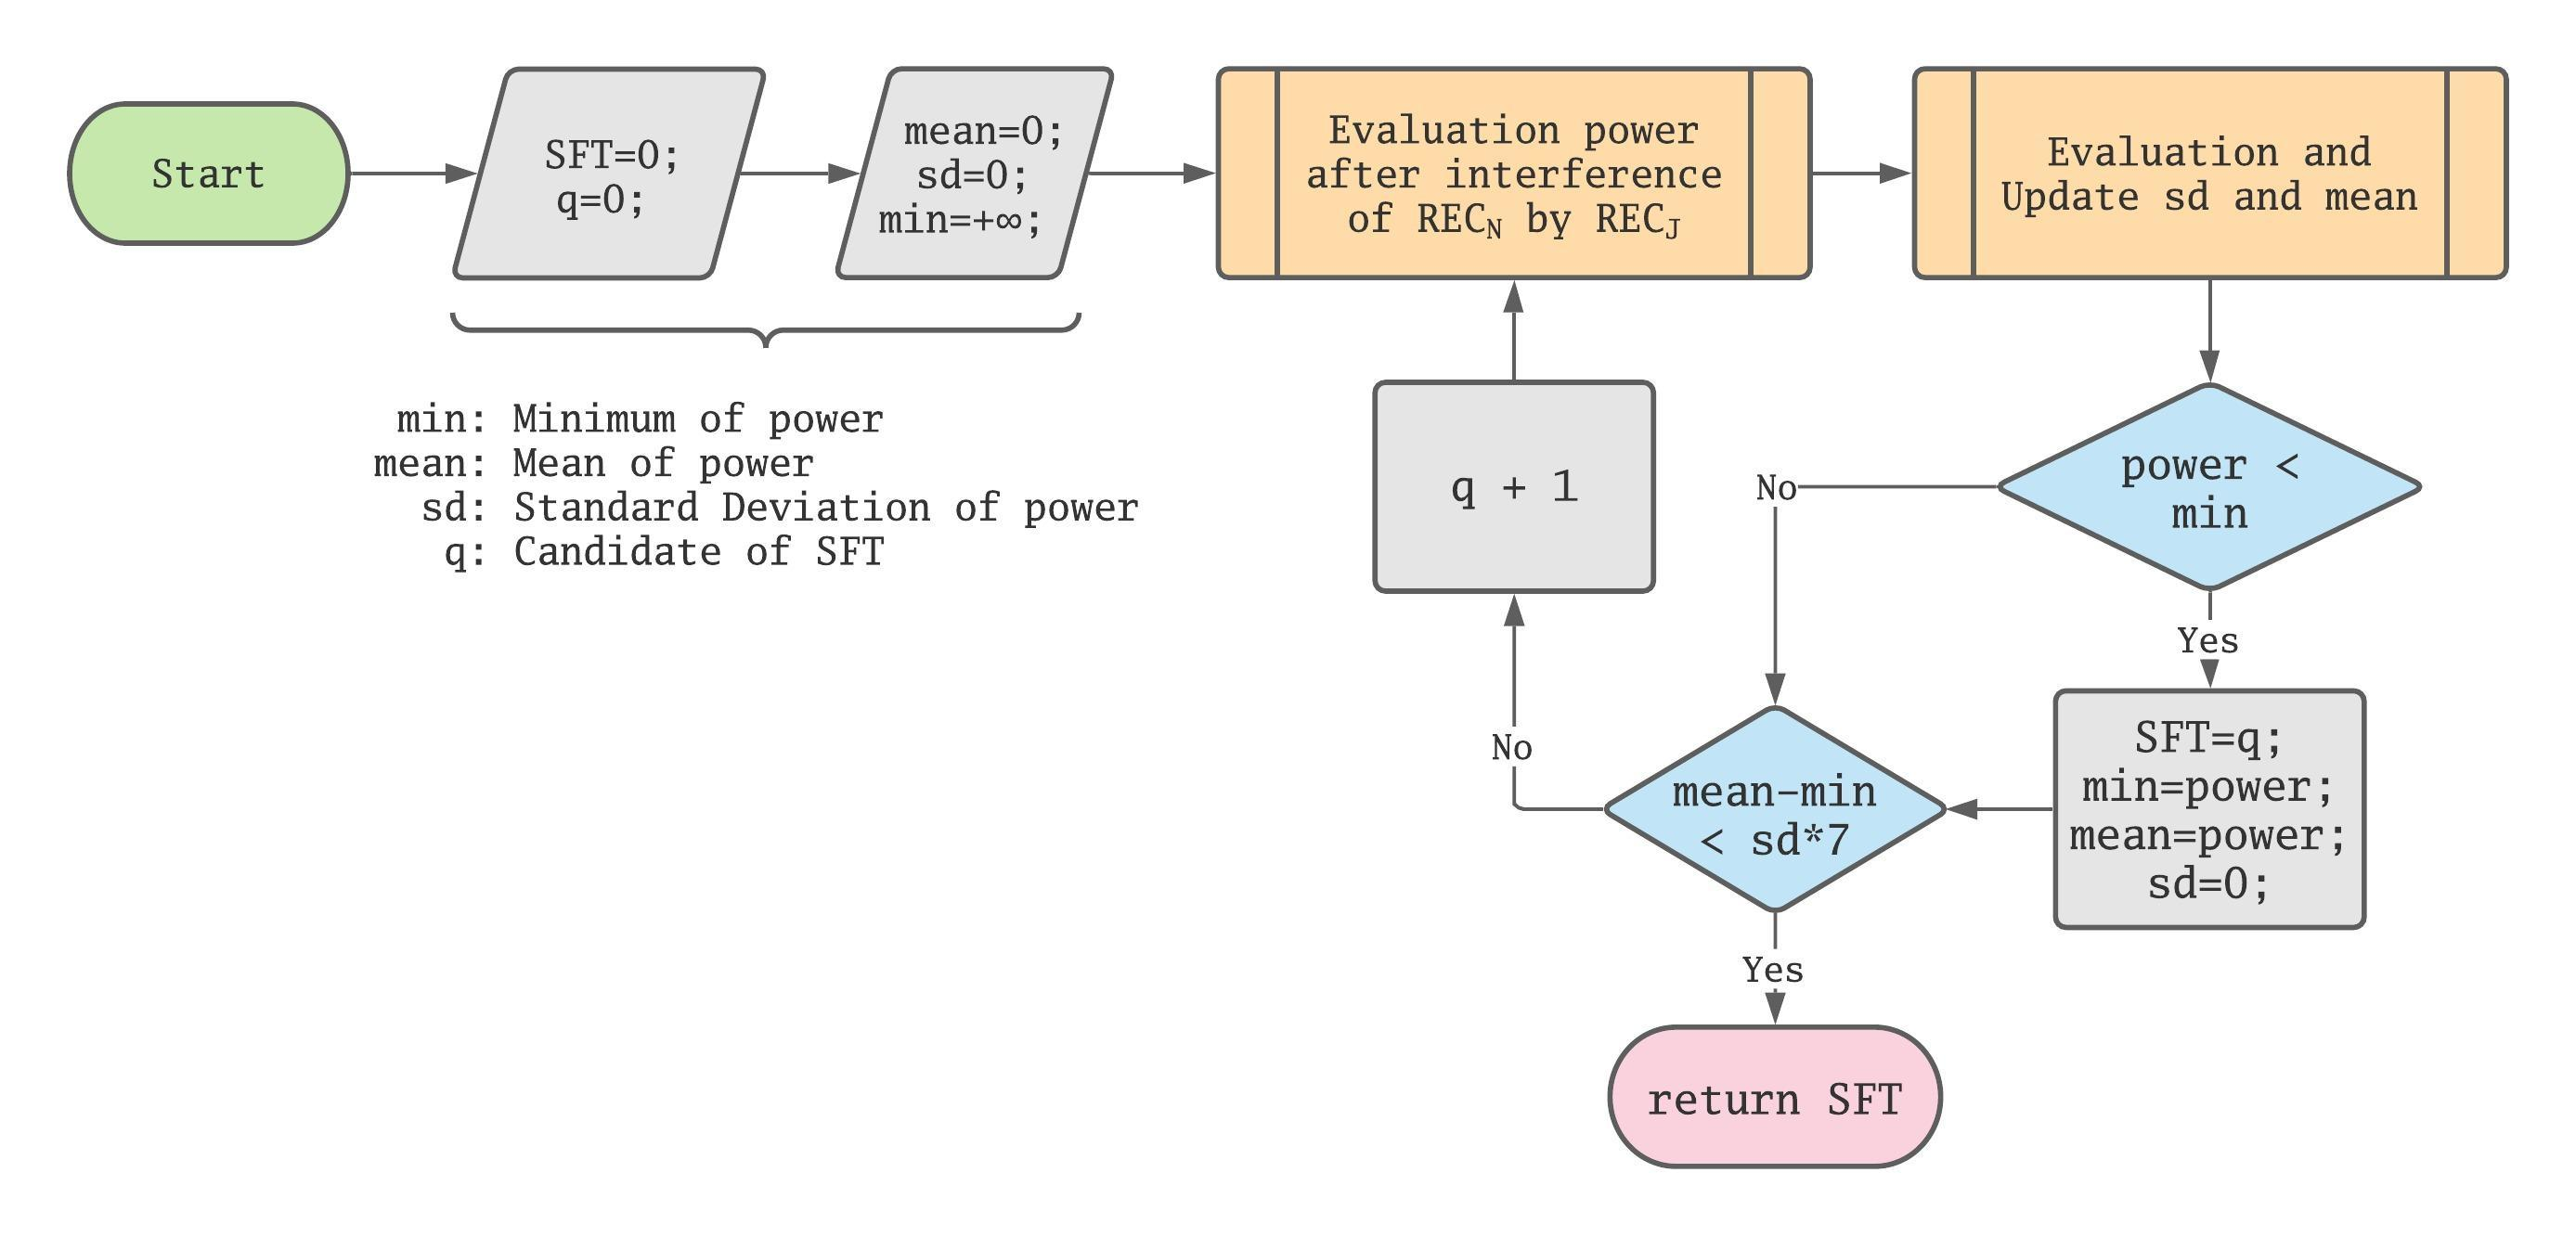
\includegraphics[width=1.0\textwidth]{estimate-shift-shift}
    \caption{聲音樣本之離散時間誤差推估演算法}
    \label{fig:estimate-shift}
\end{figure}

\begin{figure}[H]
    \centering
    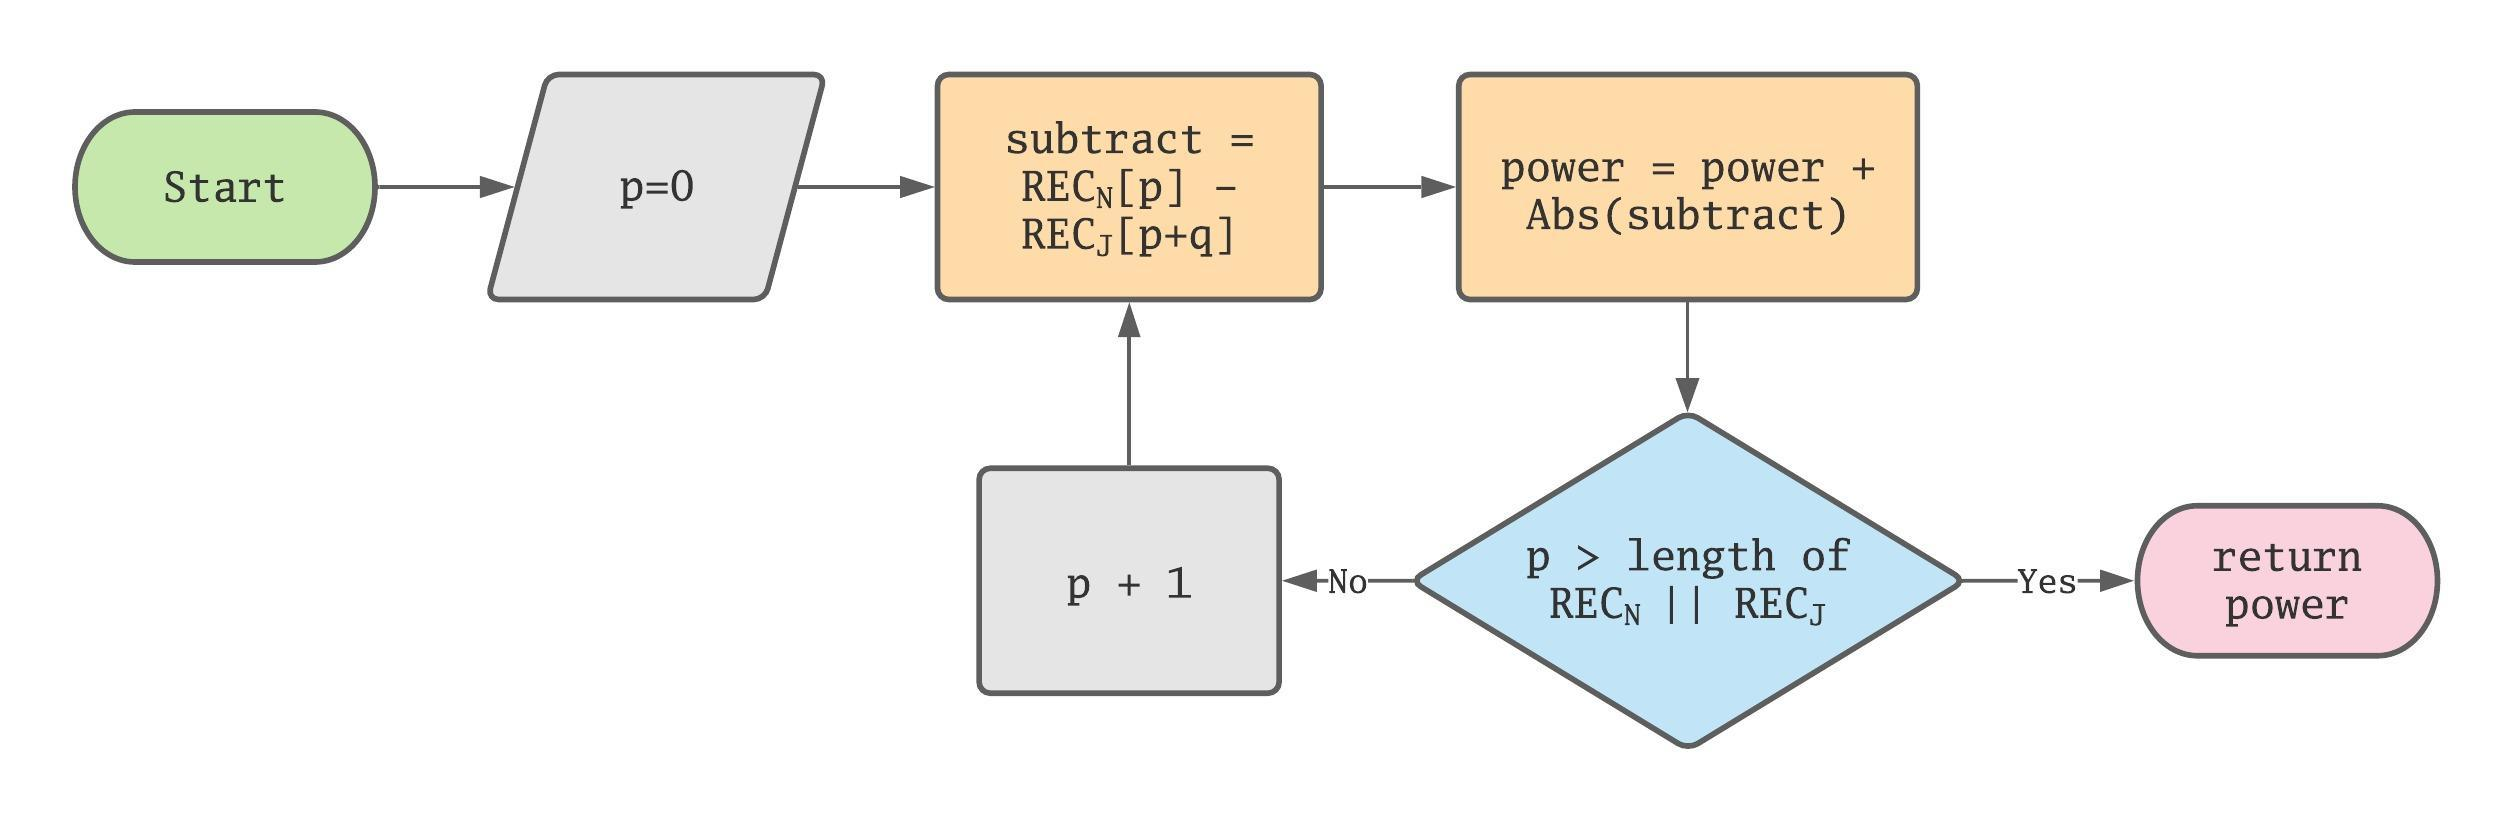
\includegraphics[width=0.95\textwidth]{estimate-shift-power}
    \caption{干涉抵銷後之總能量計算演算法}
    \label{fig:estimate-power}
\end{figure}


\section{系統理論與假設}
\label{sec:theory}

\begin{figure}[H]
    \centering
    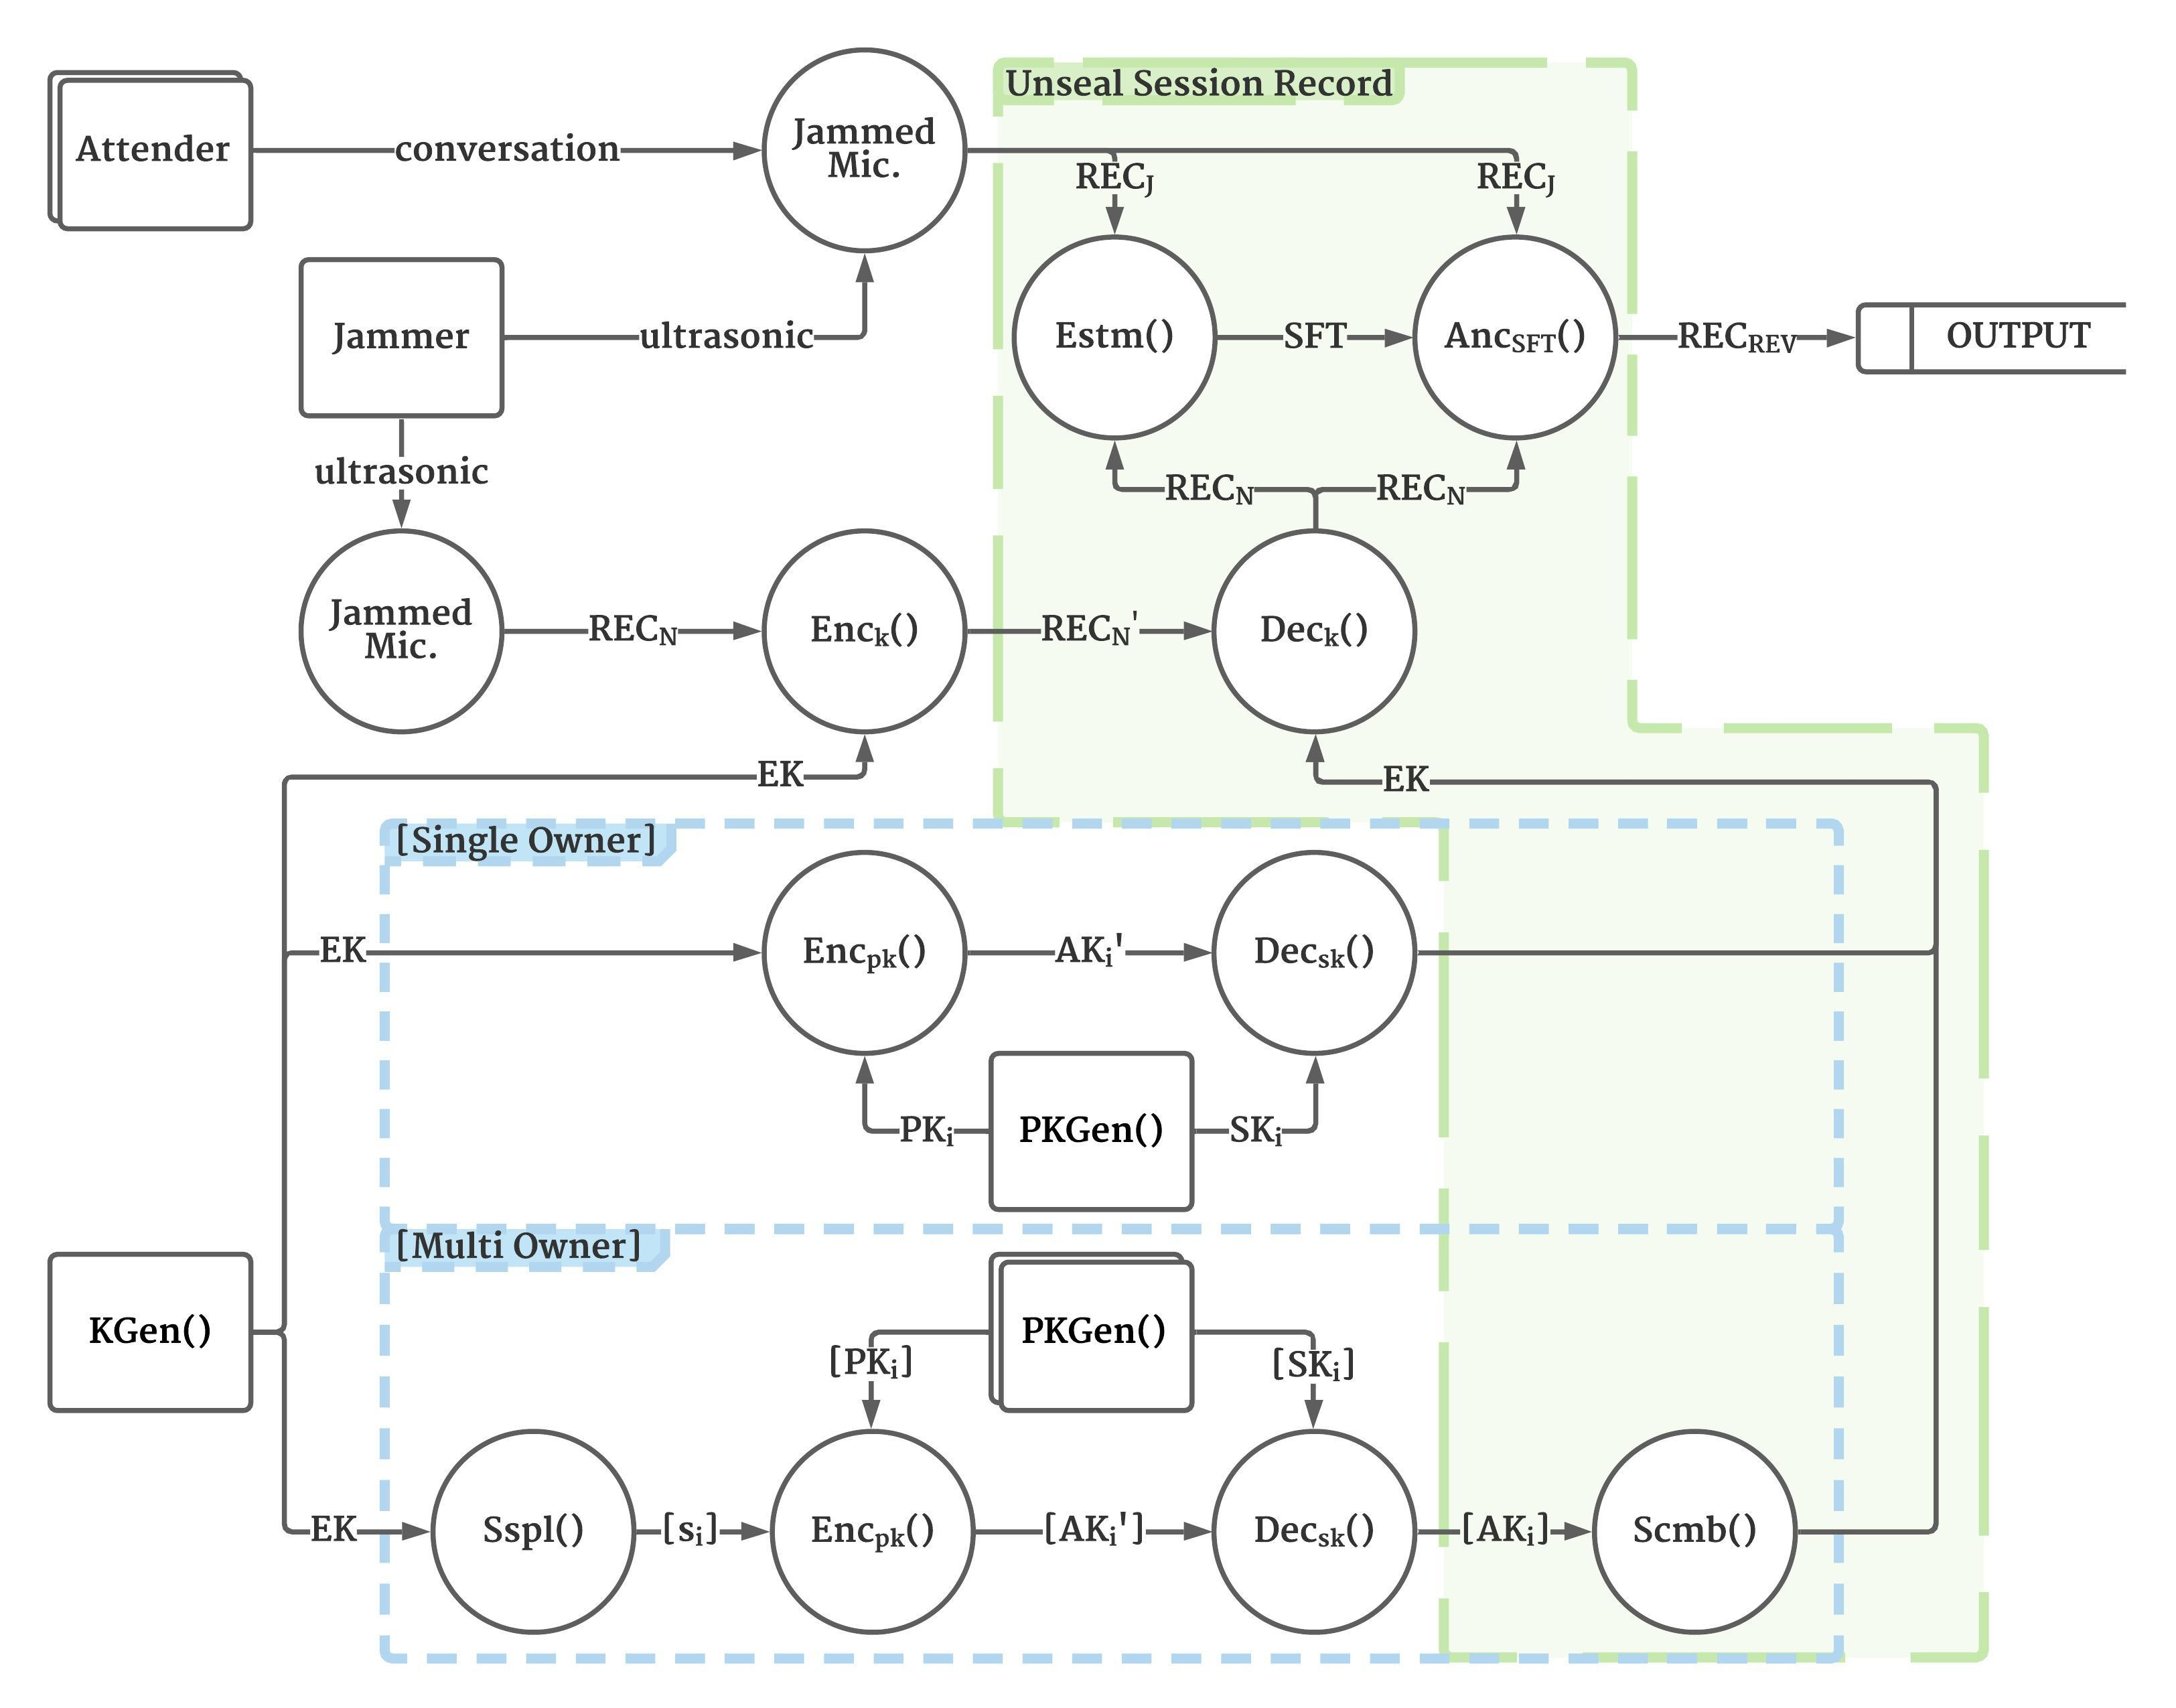
\includegraphics[width=1.0\textwidth]{system-data-flow}
    \caption{系統資料流程圖}
    \label{fig:system-data-flow}
\end{figure}
